\documentclass{report}

% Packages nécessaires
\usepackage[utf8]{inputenc}
\usepackage[T1]{fontenc}
\usepackage[french]{babel}
\usepackage{titlesec}
\usepackage{tocloft}
\usepackage{graphicx}
\usepackage{float} % pour l'option de placement [H]
\usepackage{wrapfig}   % Pour l'enroulement du texte autour des images
\usepackage{array}

% Couleurs et tableaux
\usepackage[table]{xcolor}  % Pour les couleurs de fond des lignes et en-têtes
\definecolor{headerblue}{RGB}{26, 54, 93}   % Bleu marine corporate
\definecolor{rowlight}{RGB}{245, 247, 250}   % Gris très clair pour l'alternance

% Hyperliens stylisés
\usepackage[colorlinks=true, linkcolor=headerblue, citecolor=headerblue, urlcolor=headerblue]{hyperref}

% Mathématiques et encadrés
\usepackage{amsmath, amssymb}
\usepackage{amsthm}
\usepackage{mdframed}  % Package pour les cadres

% Configuration de la page et marges
\usepackage[a4paper, left=2.5cm, right=2.5cm, top=2.5cm, bottom=2.5cm]{geometry}
\usepackage{booktabs}       % Pour des bordures nettes et professionnelles
\usepackage{tabularx}       % Pour adapter automatiquement la largeur du tableau

% En-têtes et pieds de page personnalisés (fancyhdr)
\usepackage{fancyhdr}
\setlength{\headheight}{15pt}
\pagestyle{fancy}
\fancyhf{} % Réinitialise les en-têtes et pieds de page

% En-tête : nom du chapitre à gauche et ligne fine
\fancyhead[L]{\small\itshape\nouppercase{\leftmark}}
\renewcommand{\headrulewidth}{0.4pt}

% Pied de page : ligne horizontale fine et numéro de page encadré
\renewcommand{\footrulewidth}{0.4pt}
\fancyfoot[C]{\setlength{\fboxsep}{3pt}\fbox{\footnotesize\bfseries\thepage}}

% Style pour les premières pages de chapitres (style 'plain')
\fancypagestyle{plain}{
    \fancyhf{}
    \renewcommand{\headrulewidth}{0pt}
    \renewcommand{\footrulewidth}{0.4pt}
    \fancyfoot[C]{\setlength{\fboxsep}{3pt}\fbox{\footnotesize\bfseries\thepage}}
}



% Environnements pour les théorèmes, définitions et preuves
\newtheorem{theorem}{Théorème}
\newtheorem{definition}{Définition}
\newtheorem{example}{Exemple}
\newtheorem{property}{Propriété}

\renewcommand{\contentsname}{Table des matières}
\newmdtheoremenv{boxedproperty}{Propriété}[section]  % Crée un environnement encadré pour les propriétés



% Pour avoir le petit dessin de l'INSA en bas à droite de chaque page
% \usepackage{background}
% \backgroundsetup{
% scale=1,
% angle=0,
% opacity=1,
% color=black,
% contents={\begin{tikzpicture}[remember picture,overlay]
% \node at ([xshift=-0.8in,yshift=0.8in] current page.south east) % Adjust the position of the logo.
% {\includegraphics[scale=0.8]{images/pattern.png}}; % logo goes here
% \end{tikzpicture}}
% }


% Configuration des titres des sections et sous-sections
\titleformat{\chapter}[display]
  {\normalfont\huge\bfseries}{\chaptertitlename\ \thechapter}{18pt}{\Huge}
\titleformat{\section}
  {\normalfont\Large\bfseries}{\thesection}{1em}{}
\titleformat{\subsection}
  {\normalfont\large\bfseries}{\thesubsection}{1em}{}

% Configuration de la table des matières
\renewcommand{\cftchapfont}{\bfseries}
\renewcommand{\cftsecfont}{\normalfont}
\renewcommand{\cftsubsecfont}{\normalfont}
\renewcommand{\cftchappagefont}{\bfseries}
\renewcommand{\cftsecpagefont}{\normalfont}
\renewcommand{\cftsubsecpagefont}{\normalfont}
\setlength{\cftbeforetoctitleskip}{0pt}
\setlength{\cftaftertoctitleskip}{10pt}
\renewcommand{\contentsname}{Table des matières}


\begin{document}

% --- Page de titre ---
\begin{titlepage}
    \centering
    
    \noindent
    \begin{minipage}{0.3\textwidth}
        
\includegraphics[width=0.6\linewidth]{images/logo_ensa.jpg} % Logo ENSA Tanger
    \end{minipage}%
    \hfill
    \begin{minipage}{0.5\textwidth}
        \flushright
        
\includegraphics[width=0.6\linewidth]{images/logo_sebn.jpg} % Logo SEBN-MA
    \end{minipage}

    \vspace*{3cm}
    {\Large \textbf{Rapport de Projet de Fin d'Année (PFA)} \par}
    \vspace{1cm}
    {\Huge\bfseries Application de suivi et de génération des KPIs \par}
    \vspace{0.5cm}
    {\huge (HCM-S CIM3) \par}
    
    \vspace{2.5cm}
    % --- Section "Réalisé par" et "Encadré par" côte à côte ---
    \noindent
    \begin{minipage}[t]{0.45\textwidth}
        \centering \Large
        \textbf{Réalisé par :}\\ 
        Salman EL-GHRICH
    \end{minipage}%
    \hspace{1.4cm} % <-- Tu peux modifier cette valeur pour écarter ou rapprocher les noms
    \begin{minipage}[t]{0.45\textwidth}
        \centering \Large
        \textbf{Encadré par :}\\ 
        Mr. Mouhssine Aouam
    \end{minipage}
    \par
    \vspace{2cm}

    {\large \textbf{Filière :}\\ 2ème année Cycle Ingénieur – Génie Informatique \par}
    \vspace{1.5cm}
    {\large Du 03/07/2026 au 03/09/2026 \par} % Ajout des dates ici
    \vspace{1cm}
    
    \vfill
    {\Large \textbf{Entreprise d'accueil : SEBN-MA} \par}
    \vspace{1cm}
    {\large Année Universitaire : 2025-2026 \par}
\end{titlepage}

% --- Numérotation des pages préliminaires (chiffres romains : i, ii, iii...) ---
\cleardoublepage
\pagenumbering{roman}
\setcounter{page}{1}

\chapter*{Avant-propos}
\addcontentsline{toc}{chapter}{Avant-propos} % Pour l'ajouter à la table des matières
\large \noindent
Le présent travail est réalisé par \textbf{Salman EL-GHRICH}, étudiant en 2ème année du cycle ingénieur, filière \textbf{Génie Informatique}, à l'\textbf{École Nationale des Sciences Appliquées de Tanger (ENSA Tanger)}, dans le cadre du stage de Projet de Fin d'Année (PFA).

\vspace{1cm}

\begin{description}
    \item[\Large Intitulé du projet :] \hfill \\
    \vspace{0.2cm}
    Application de suivi et de génération des KPIs (HCM-S CIM3)
    
    \vspace{1.5cm}
    
    \item[\Large Établissement d'accueil :] \hfill \\
    \textbf{Entreprise :} SE BORDNETZE MOROCCO S.A.R.L (SEBN-MA)\\
    \textbf{Adresse :} Tangier Free Zone - TFZ, Lot 32, MA 90 000\\
    \textbf{Téléphone :} +212 5 39 39 93 04
    
    
    \vspace{1.5cm}
    \item[\Large Encadrant professionnel :] \hfill \\
    \textbf{Mr. Mouhssine Aouam} — Process & New technologies Group Leader (Tuteur et encadrant de stage)
    
    \vspace{1.5cm}
    
    \item[\Large Période du stage :] \hfill \\
    \textbf{Début :} 03/07/2026 \\
    \textbf{Fin :} 03/09/2026
\end{description}
\chapter*{Dédicaces}
\addcontentsline{toc}{chapter}{Dédicaces} % Ajout à la table des matières

\begin{flushright}
    \textit{Je dédie ce modeste travail...}
\end{flushright}

\vspace{1cm}

\noindent \textbf{À mes chers parents,}\\
Aucune dédicace ne saurait exprimer toute la profondeur de ma gratitude. Merci d'avoir toujours été là pour moi, de m'avoir soutenu dans chaque étape de ma vie et d'avoir cru en moi. Ce travail est le fruit de vos sacrifices, de vos encouragements constants. Merci pour tout.
\vspace{1cm}


\noindent \textbf{À mes chers frères,}\\
Pour votre soutien indéfectible, votre complicité précieuse et votre présence rassurante à chaque étape de ma vie. Merci pour vos encouragements constants. Que nos liens de fraternité demeurent toujours aussi solides.



\chapter*{Remerciements}
\addcontentsline{toc}{chapter}{Remerciements}

Au terme de ce projet, je tiens à exprimer ma profonde gratitude à toutes les personnes qui ont contribué, de près ou de loin, à son aboutissement et à sa réussite.

\vspace{0.4cm}

Je remercie en premier lieu \textbf{Dieu} le Tout-Puissant de m'avoir accordé la force, la patience et la volonté nécessaires pour mener à bien ce travail.

\vspace{0.4cm}

J'exprime mes vifs remerciements à l'entreprise \textbf{SEBN-MA} pour son accueil chaleureux et pour m'avoir offert l'opportunité d'effectuer ce stage dans un environnement professionnel stimulant.

\vspace{0.4cm}

Mes sincères remerciements s'adressent tout particulièrement à mon encadrant professionnel, \textbf{M. Mouhssine AOUAM}, pour sa disponibilité constante malgré la pression du travail, ses précieux conseils, ses orientations avisées et la confiance qu'il m'a accordée tout au long de cette expérience.

\vspace{0.4cm}

Je tiens également à remercier le corps professoral et l'équipe pédagogique de l'\textbf{ENSA Tanger} pour la qualité de la formation et l'excellence du cadre d'apprentissage dispensé tout au long de mon cursus d'ingénieur.

\chapter*{Liste des abréviations}
\addcontentsline{toc}{chapter}{Liste des abréviations}

\vspace{0.5cm}

% Configuration de l'alternance des couleurs des lignes
\rowcolors{2}{rowlight}{white}

\noindent
\begin{tabularx}{\textwidth}{>{\bfseries}p{3cm} X}
    \toprule
    % En-tête du tableau avec fond coloré et texte blanc
    \rowcolor{headerblue} 
    \textcolor{white}{\textbf{Abréviation}} & \textcolor{white}{\textbf{Signification}} \\
    \midrule
    
    % --- Contexte Industriel & Entreprise ---
    SEBN-MA   & Sumitomo Electric Bordnetze Morocco \\
    CMF       & Central Manufacturing \\
    HCM-S     & Hyper Compact Machine – Set bar \\
    CIM-3     & Compact Insertion Machine III \\
    KPI       & Key Performance Indicator (Indicateur Clé de Performance) \\
    OEE       & Overall Equipment Effectiveness (Taux de Rendement Synthétique - TRS) \\
    DSI       & Direction des Systèmes d'Information \\
    
    % --- Contexte Académique ---
    PFA       & Projet de Fin d'Année \\
    ENSA-T    & École Nationale des Sciences Appliquées de Tanger \\
    
    % --- Contexte Informatique & DevOps ---
    API       & Application Programming Interface \\
    BDD       & Base de Données \\
    CI / CD   & Continuous Integration / Continuous Deployment \\
    CRUD      & Create, Read, Update, Delete \\
    DTO       & Data Transfer Object \\
    JWT       & JSON Web Token \\
    MVC       & Modèle - Vue - Contrôleur \\
    ORM       & Object-Relational Mapping \\
    REST      & Representational State Transfer \\
    SPA       & Single Page Application \\
    TLS / SSL & Transport Layer Security / Secure Sockets Layer \\
    UI / UX   & User Interface / User Experience \\
    UML       & Unified Modeling Language \\
    WAF       & Web Application Firewall \\
    
    \bottomrule
\end{tabularx}

% --- Résumé (Français) ---
\cleardoublepage
\phantomsection
\chapter*{Résumé}
\addcontentsline{toc}{chapter}{Résumé}
\markboth{Résumé}{Résumé}

Dans le cadre de l'industrie automobile de Rang~1, l'efficacité des lignes d'assemblage repose sur un suivi rigoureux des indicateurs clés de performance (\textit{KPIs}). Ce Projet de Fin d'Année, mené au sein de l'entreprise \textbf{SEBN-MA} (site de Tanger Free Zone), porte sur la conception, le développement et le déploiement d'une plateforme logicielle moderne dédiée au pilotage des ensembles de machines synchronisées \textbf{HCM-S CIM-3}.

Historiquement, la collecte et la mise en forme de ces indicateurs reposaient sur des classeurs Excel isolés et des manipulations manuelles chronophages, limitant la visibilité en temps réel et exposant les données à des risques d'erreurs humaines. Pour répondre à ces défis, nous avons développé une application web découplée articulée autour d'un client réactif en \textbf{React~19} (TypeScript, Tailwind CSS~v4, TanStack Query, Chart.js) et d'un serveur d'API REST asynchrone haute performance propulsé par \textbf{FastAPI}, \textbf{SQLAlchemy~2.0} et une base de données relationnelle \textbf{PostgreSQL} (\texttt{asyncpg}).

L'application intègre notamment un module novateur d'importation en masse (\textit{Bulk Data Entry}) capable de parser instantanément les données copiées depuis le presse-papiers Excel, avec validation dynamique des plages de semaines et des équipements. La sécurité repose sur une authentification JWT à double jeton (avec rafraîchissement transparent sous Axios) et un stockage \textit{Zero-Knowledge} (SHA-256) des clés d'API destinées à l'automatisation de l'ingestion (Phase~2). 

La fiabilité du système est attestée par une suite de \textbf{151 tests automatisés} exécutés avec un taux de réussite de 100\,\% sous Vitest et Pytest. L'infrastructure est conteneurisée via un \textit{Multi-stage Dockerfile} (réduisant le poids de l'image de production à environ 180~Mo) et validée par un pipeline d'intégration continue (\textit{CI/CD}) sous GitHub Actions avec un temps de compilation de 9,3~secondes. La solution garantit ainsi à SEBN-MA un gain de temps opérationnel substantiel, une intégrité totale des données industrielles et une transition fluide vers l'Usine du Futur (Industrie~4.0).

\vspace{0.6cm}
\noindent \textbf{Mots-clés :} Indicateurs de Performance (KPIs), OEE / TRS, HCM-S CIM-3, Industrie 4.0, FastAPI, React 19, PostgreSQL, Docker, Intégration Continue (CI/CD), SEBN-MA.

% --- Abstract (English) ---
\cleardoublepage
\phantomsection
\chapter*{Abstract}
\addcontentsline{toc}{chapter}{Abstract}
\markboth{Abstract}{Abstract}

In Tier-1 automotive manufacturing, production line efficiency heavily relies on the rigorous monitoring of Key Performance Indicators (\textit{KPIs}). This engineering project, conducted at \textbf{SEBN-MA} (Tangier Free Zone plant), focuses on designing, developing, and deploying a modern web application dedicated to supervising \textbf{HCM-S CIM-3} synchronized machine sets.

Historically, KPI aggregation relied on isolated Excel workbooks and time-consuming manual workflows, hindering real-time visibility and risking data inconsistency. To overcome these limitations, we engineered a decoupled web platform featuring a reactive \textbf{React~19} frontend (TypeScript, Tailwind CSS~v4, TanStack Query, Chart.js) and a high-performance asynchronous REST API powered by \textbf{FastAPI}, \textbf{SQLAlchemy~2.0}, and \textbf{PostgreSQL} (\texttt{asyncpg}).

Key achievements include a \textit{Bulk Data Entry} feature that parses raw Excel clipboard data with real-time validation, dual-token JWT authentication with silent refresh, and \textit{Zero-Knowledge} SHA-256 API key hashing for automated ingestion. Quality assurance is backed by \textbf{151 automated tests} (100\% pass rate on Vitest and Pytest), multi-stage Docker packaging ($\approx$180~MB image size), and a GitHub Actions CI/CD pipeline achieving a 9.3-second build time. This solution delivers significant time savings, rock-solid data integrity, and a concrete step toward Industry 4.0 for SEBN-MA.

\vspace{0.6cm}
\noindent \textbf{Keywords :} KPIs, OEE, HCM-S CIM-3, Industry 4.0, Automotive Wiring Harness, FastAPI, React 19, PostgreSQL, Docker, CI/CD, SEBN-MA.

% --- Table des matières ---
\cleardoublepage
\phantomsection
\tableofcontents

% --- Personnalisation du titre (si non géré par babel) ---
\renewcommand{\listfigurename}{Liste des figures}

% --- Génération automatique de la liste des figures ---
\cleardoublepage
\phantomsection
\addcontentsline{toc}{chapter}{\listfigurename}
\listoffigures

% --- Numérotation du corps du rapport (chiffres arabes : 1, 2, 3...) ---
\cleardoublepage
\pagenumbering{arabic}
\setcounter{page}{1}

% --- Inclusion des chapitres ---
\chapter{Présentation de l'entreprise d'accueil - SEBN-MA}
\label{chap:presentation_entreprise}

\section*{Introduction}
\addcontentsline{toc}{section}{Introduction}
Dans ce chapitre, je commencerai par une présentation de l'entreprise d'accueil, de sa structure intérieure, de ses clients et de ses réalisations. Une deuxième partie de ce chapitre concerne une analyse détaillée du cycle de production de l'usine, en mettant l'accent sur les différentes étapes et les technologies utilisées pour optimiser l'efficacité et la qualité de la production.

% ---------------------------------------------------------
\section{Présentation générale de l'entreprise}

\subsection{Nom et identité juridique}
L'entreprise d'accueil se nomme \textbf{SUMITOMO ELECTRIC BORDNETZE Morocco (SEBN-MA)}. Il s'agit d'une Société à Responsabilité Limitée à Associé Unique (SARL AU), filiale du groupe japonais Sumitomo Wiring Systems (SWS), dont le capital social s'élève à 140 000 000 d'euros.

Créée en 2001, SEBN-MA est spécialisée dans la conception et la fabrication de faisceaux électriques destinés à l'industrie automobile. Grâce à son expertise et à son savoir-faire, l'entreprise fournit plusieurs grands constructeurs automobiles internationaux et contribue au développement du secteur automobile au Maroc.

Mon stage s'est déroulé sur le site de Tanger, où sont réalisées les différentes opérations de production, d'assemblage et de contrôle des faisceaux électriques.

\subsection{Secteur d'activité}
SEBN opère dans le secteur du câblage automobile, en tant que fournisseur de Rang 1 (Tier 1). Cela signifie que l'entreprise livre directement les KSK, Autarkies, Batteries \& HV, sans intermédiaire. Le groupe est certifié selon les normes IATF 16949 (management de la qualité dans l'automobile), ISO 9001 et ISO 14001 (management environnemental), ISO 45001:2018 (management de la santé et de la sécurité au travail).

\subsection{Localisation}
SE Bordnetze Morocco (SEBN-MA) dispose de plusieurs sites de production au Maroc, notamment à Tanger Free Zone (TFZ), Tanger Automotive City (TAC) et Bouknadel (Salé).

Le site de Tanger Free Zone, où s'est déroulé mon stage, est implanté dans la région de Tanger-Tétouan-Al Hoceïma. Grâce à cette localisation stratégique et à la complémentarité de ses différents sites industriels, SEBN-MA assure efficacement la production et l'approvisionnement de nombreux constructeurs automobiles européens, tout en répondant aux exigences de qualité, de coût et de délai de ses clients.

Bien que les trois sites exercent la même activité principale, à savoir la fabrication de faisceaux électriques destinés à l'industrie automobile, le présent rapport porte exclusivement sur le site de Tanger Free Zone (TFZ).

\begin{figure}[H]
    \centering
    % Remplace 'nom_de_l_image.png' par ton fichier
    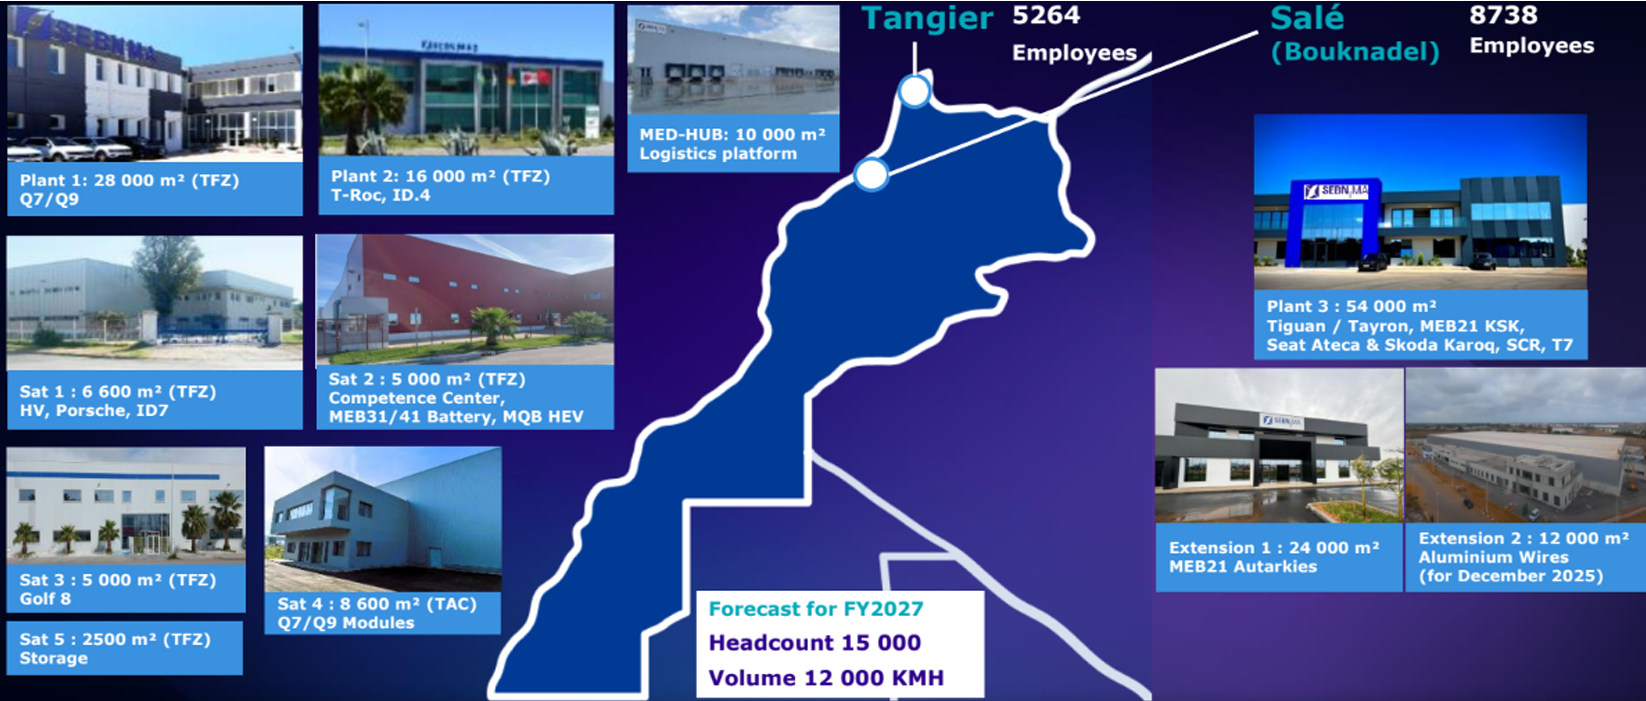
\includegraphics[width=0.7\textwidth]{images/Ch1/01.png} 
    \caption{Zone géographique de SEBN-MA} 
    \label{fig:zone_geo_sebn}
\end{figure}

\subsection{Certifications et achèvements}
SEBN-MA accorde une grande importance à la qualité, à la sécurité et à l'amélioration continue de ses processus. Grâce à son engagement envers les normes internationales et les exigences de ses clients, l'entreprise a obtenu plusieurs certifications, notamment IATF 16949, ISO 14001 et ISO 45001. Elle a également reçu plusieurs distinctions décernées par des constructeurs automobiles tels qu'Audi, SEAT et Volkswagen, témoignant de la fiabilité de ses produits et de la performance de son système de management.
\begin{figure}[H]
    \centering
    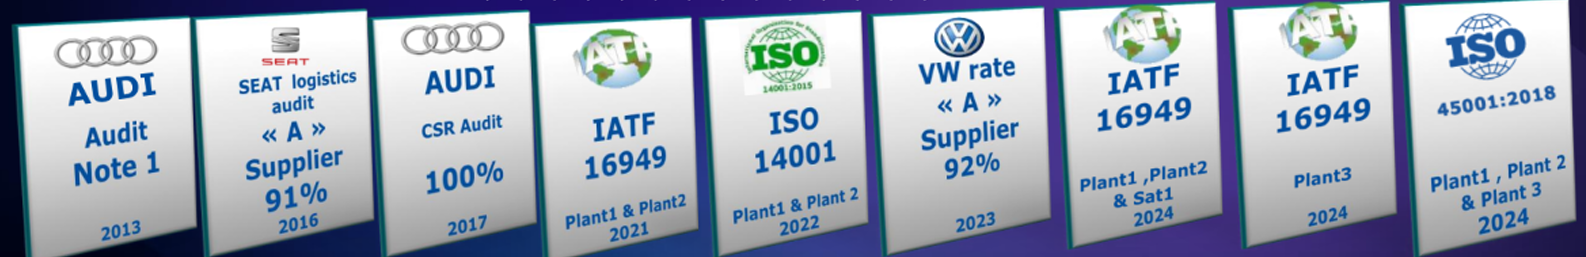
\includegraphics[width=0.7\textwidth]{images/Ch1/02.png} 
    \caption{Certifications et distinctions de SEBN-MA} 
    \label{fig:certifications_sebn}
\end{figure}

\subsection{Fiche signalétique}

% Réactivation des couleurs alternées pour ce tableau (si désactivé)
\rowcolors{2}{rowlight}{white}

\begin{table}[H]
    \centering
    \caption{Informations générales de SEBN-MA}
    \label{tab:fiche_signaletique}
    \vspace{0.3cm} % Petit espace entre le titre et le tableau
    
    % On utilise tabularx pour que le tableau prenne toute la largeur
    % La première colonne (Élément) fait 4.5cm et est en gras
    % La deuxième (Information) s'adapte automatiquement avec 'X'
    \begin{tabularx}{\textwidth}{>{\bfseries}p{4.5cm} X}
        \toprule
        % En-tête coloré
        \rowcolor{headerblue}
        \textcolor{white}{\textbf{Élément}} & \textcolor{white}{\textbf{Information}} \\
        \midrule
        
        Raison sociale    & SE Bordnetze Morocco (SEBN-MA) \\
        Forme juridique   & Société à Responsabilité Limitée à Associé Unique (SARL AU) \\
        Date de création  & 2001 \\
        Capital social    & 140 000 000 \texteuro \\ % ou "euros"
        Siège social      & Tanger Free Zone, Maroc \\
        Activité          & Fabrication de faisceaux électriques automobiles \\
        Groupe            & Sumitomo Wiring Systems (SWS) \\
        Certifications    & IATF 16949, ISO 9001, ISO 14001, ISO 45001:2018 \\
        
        \bottomrule
    \end{tabularx}
\end{table}
% ---------------------------------------------------------
\section{Historique et évolution du groupe}

\subsection{Origines}
La famille Sumitomo trouve ses origines au Japon au début du 17\up{e} siècle. Elle a été fondée par Masatomo Sumitomo, un marchand visionnaire qui a établi les bases solides de l'entreprise familiale. L'origine de la famille Sumitomo remonte aux débuts de Sumitomo House, qui a prospéré grâce au commerce du cuivre et d'autres marchandises. 

Masatomo Sumitomo a laissé derrière lui les "Préceptes du Fondateur", un ensemble de principes qui ont façonné la philosophie de Sumitomo en matière de conduite commerciale. Ces préceptes ont guidé la famille Sumitomo à travers les générations, contribuant à son succès durable et à sa réputation d'intégrité et d'engagement envers la communauté et le développement économique. Aujourd'hui, la famille Sumitomo est à la tête d'un vaste groupe d'entreprises diversifiées opérant dans différents secteurs à travers le monde.

% Affichage de deux images côte à côte pour gagner de la place et faire plus professionnel
\begin{figure}[H]
    \centering
    \begin{minipage}{0.45\textwidth}
        \centering
        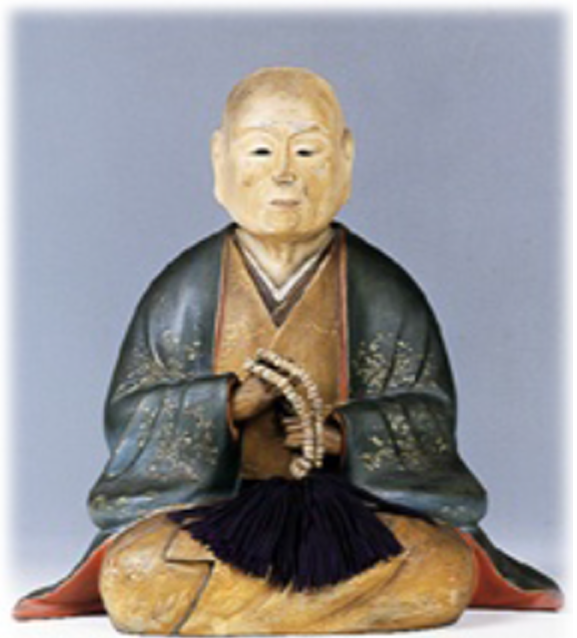
\includegraphics[width=0.9\linewidth]{images/Ch1/03.png}
        \caption{Statue en bois de Masatomo Sumitomo}
        \label{fig:statue_sumitomo}
    \end{minipage}\hfill
    \begin{minipage}{0.45\textwidth}
        \centering
        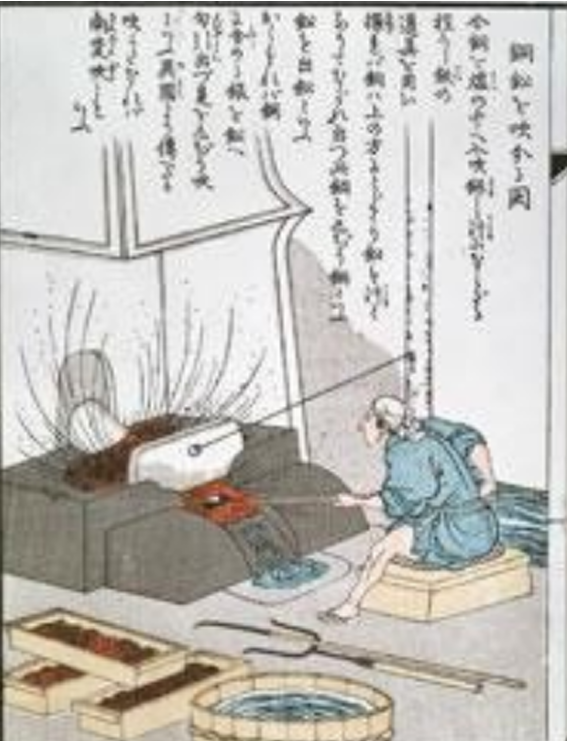
\includegraphics[width=0.9\linewidth]{images/Ch1/04.png}
        \caption{Méthode originale d'affinage du cuivre (Sumitomo Group)}
        \label{fig:affinage_cuivre}
    \end{minipage}
\end{figure}

\subsection{Le groupe Sumitomo Electric Bordnetze}
Le groupe SUMITOMO ELECTRIC BORDNETZE est un équipementier automobile spécialisé dans la fabrication des faisceaux électriques automobiles. Il a vu sa naissance pour la première fois en 1986 en tant qu'une joint-venture entre le groupe VOLKSWAGEN AG et SIEMENS AG. En effet, le groupe a été nommé pour la première fois VOLKSWAGEN BORDNETZE GMBH, alors qu'en 2006, il a poursuivi son activité sous le nom SUMITOMO ELECTRIC BORDNETZE après son rachat par le fameux groupe japonais SUMITOMO ELECTRIC INDUSTRIES.

Le groupe possède 39 sites implantés dans 13 pays, avec un siège central installé à Wolfsburg en Allemagne. De plus, le groupe emploie près de 39 000 employés de différentes nationalités.

\begin{figure}[H]
    \centering
    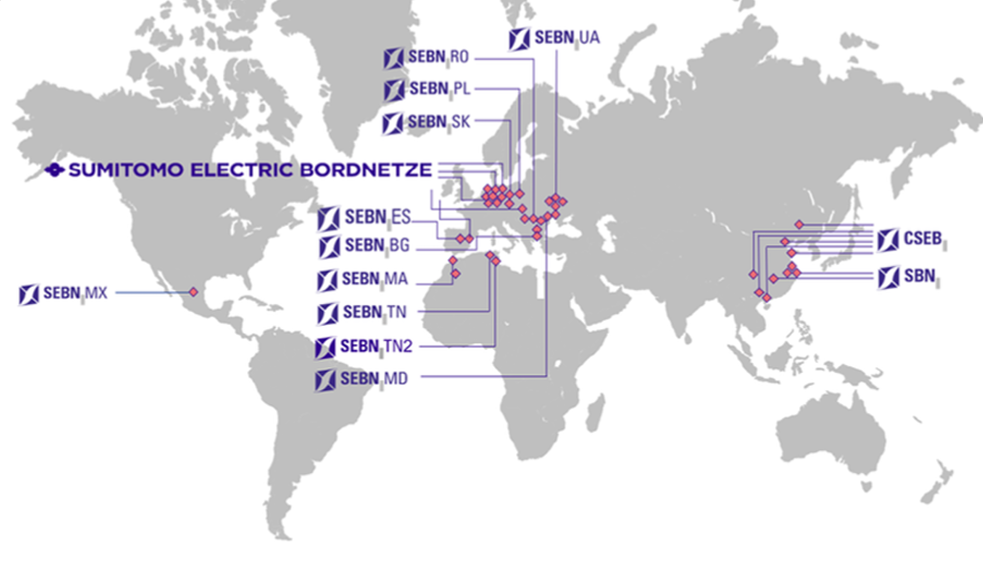
\includegraphics[width=0.8\textwidth]{images/Ch1/05.png}
    \caption{Les sites de SUMITOMO ELECTRIC BORDNETZE}
    \label{fig:sites_sebn}
\end{figure}

\subsection{L'historique de SEBN-MA}

\begin{figure}[H]
    \centering
    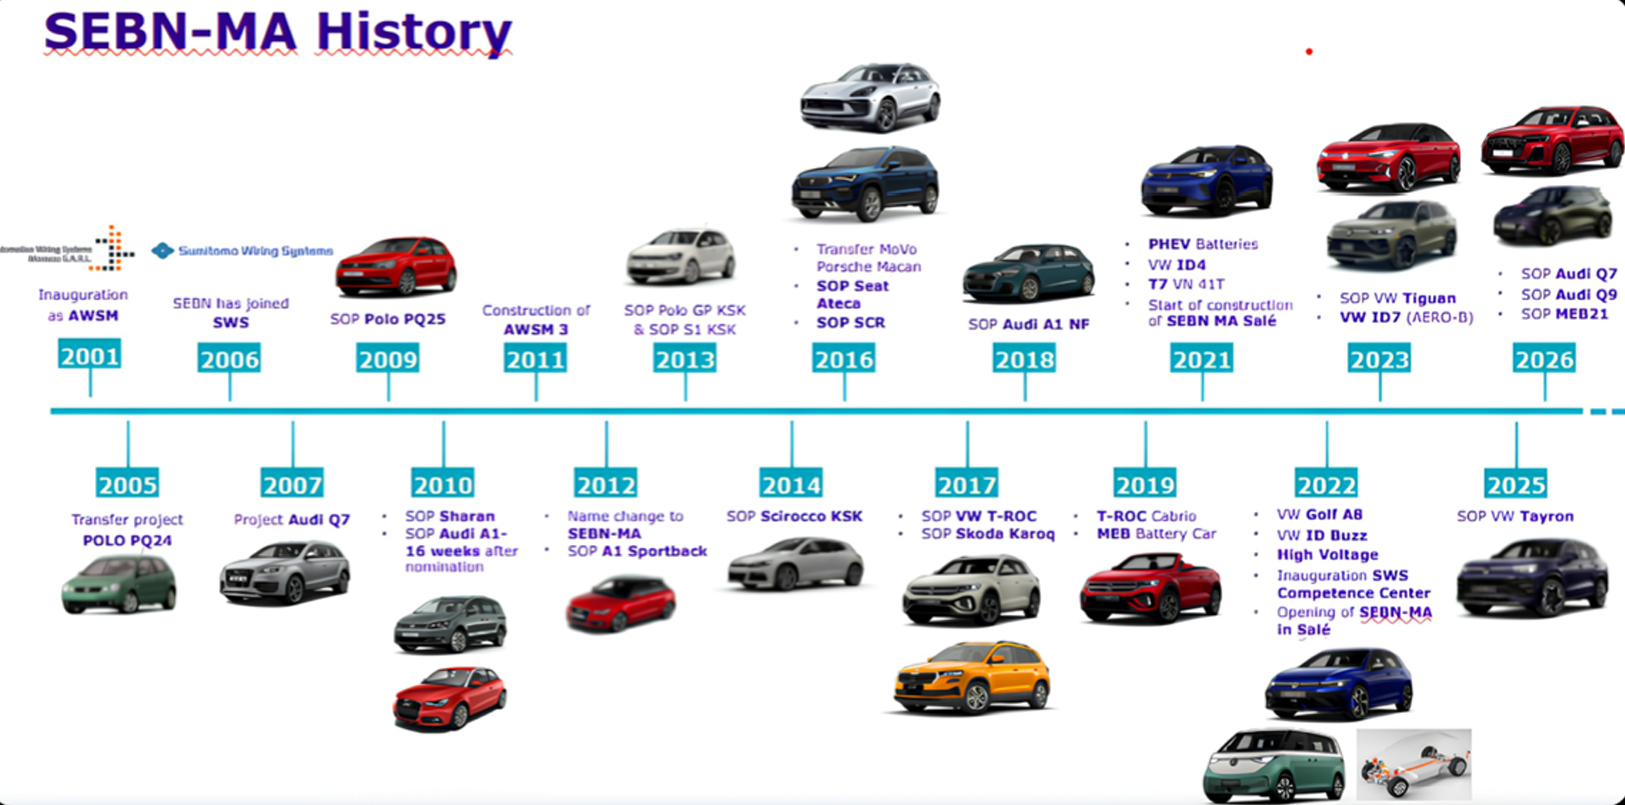
\includegraphics[width=0.85\textwidth]{images/Ch1/06.png}
    \caption{Historique de SEBN-MA}
    \label{fig:historique_sebn_ma}
\end{figure}


% ---------------------------------------------------------
\section{Activités et domaines d'intervention}

\subsection{Les différents câbles produits par SEBN-MA}
Au sein de SEBN-MA se fait la production de deux types de câbles. On trouve :

\begin{itemize}
    \item \textbf{Projet KSK :} C'est un ensemble des faisceaux de câbles électriques rassemblés dans un seul câble qui sera lié directement au moteur et qui contient essentiellement les câbles de base comme celui du frein, des feux, etc., plus les spécifications des clients. C'est le câble principal de la voiture.
    \begin{itemize}
        \item \textit{KSK INRA :} Partie compartiment.
        \item \textit{KSK MORA :} Partie moteur.
    \end{itemize}
    
    \item \textbf{Les projets Autarks :} Ce sont des faisceaux de câbles des équipements et des options de voitures telles que les portières, les vitres, les sièges, l'Airbag...
\end{itemize}

\begin{figure}[H]
    \centering
    \begin{minipage}{0.45\textwidth}
        \centering
        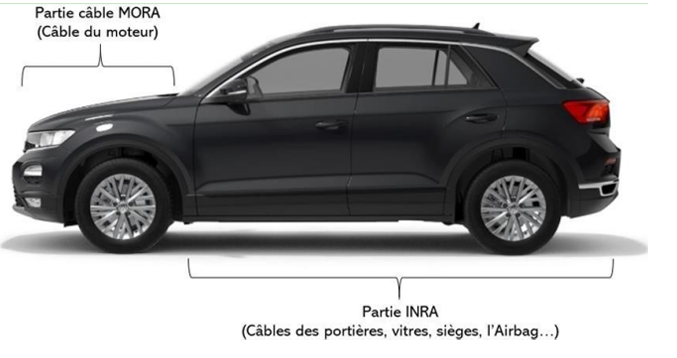
\includegraphics[width=0.9\linewidth]{images/Ch1/07.png}
        \caption{Partie câble MORA et INRA de voiture T-ROC}
        \label{fig:cable_mora_inra}
    \end{minipage}\hfill
    \begin{minipage}{0.45\textwidth}
        \centering
        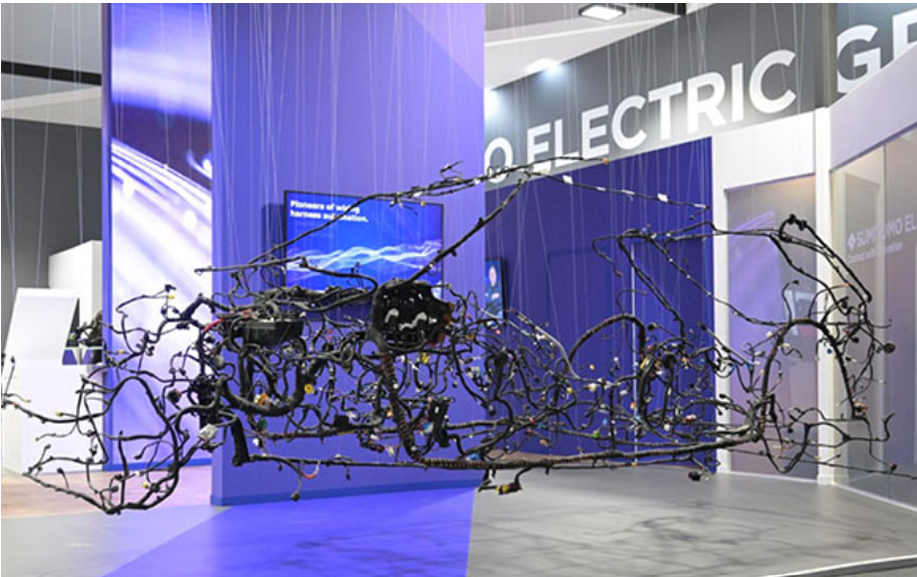
\includegraphics[width=0.9\linewidth]{images/Ch1/08.png}
        \caption{Exemple d'un faisceau électrique (KSK)}
        \label{fig:faisceau_ksk}
    \end{minipage}
\end{figure}

\subsection{Produits et Clients de SEBN-MA}
SE Bordnetze Morocco (SEBN-MA) est spécialisée dans la fabrication de faisceaux électriques destinés à l'industrie automobile. La filiale marocaine produit principalement trois familles de produits : les faisceaux électriques conventionnels (KSK), les systèmes électriques autonomes (Autarkies) ainsi que les faisceaux destinés aux véhicules électriques et hybrides, notamment les systèmes High Voltage (HV) et les ensembles de batteries.

\begin{figure}[H]
    \centering
    \begin{minipage}{0.45\textwidth}
        \centering
        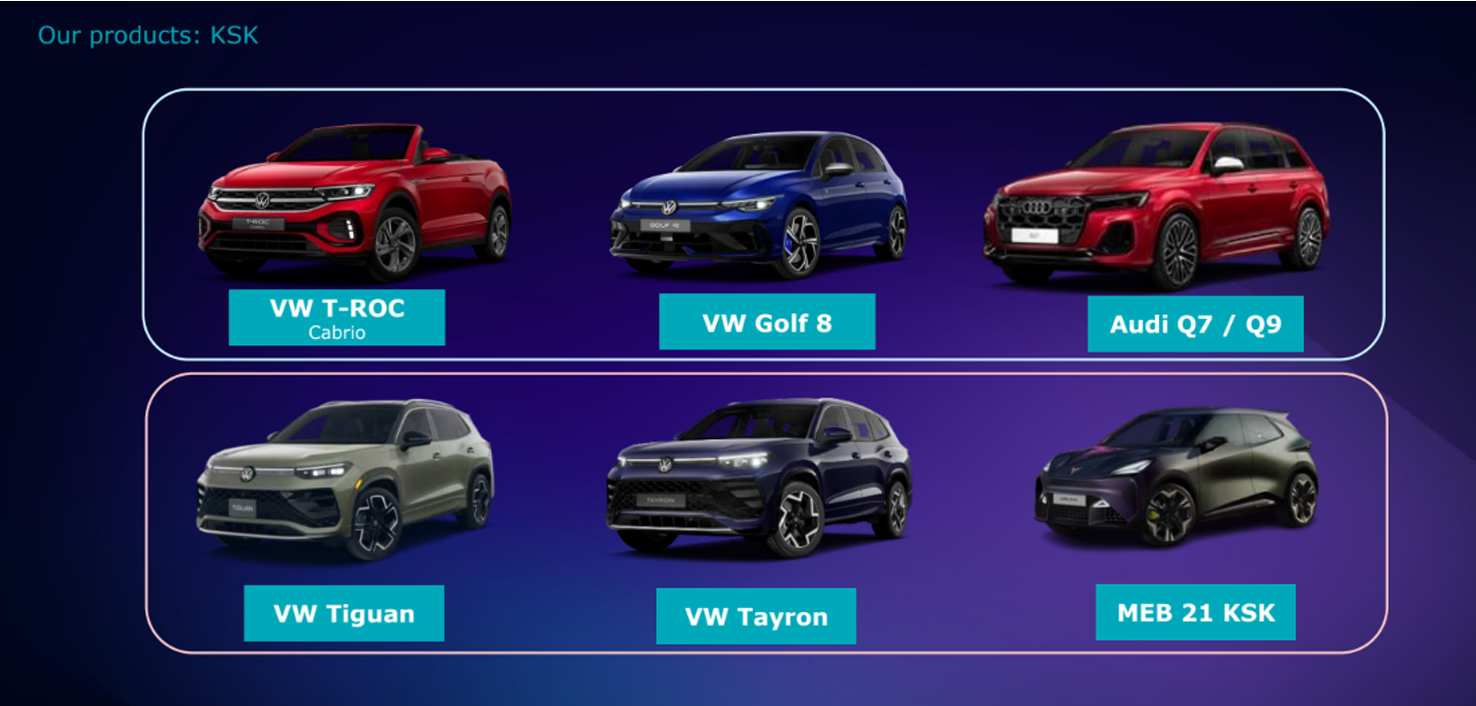
\includegraphics[width=0.9\linewidth]{images/Ch1/09.png}
        \caption{Les produits de KSK}
        \label{fig:produits_ksk}
    \end{minipage}\hfill
    \begin{minipage}{0.45\textwidth}
        \centering
        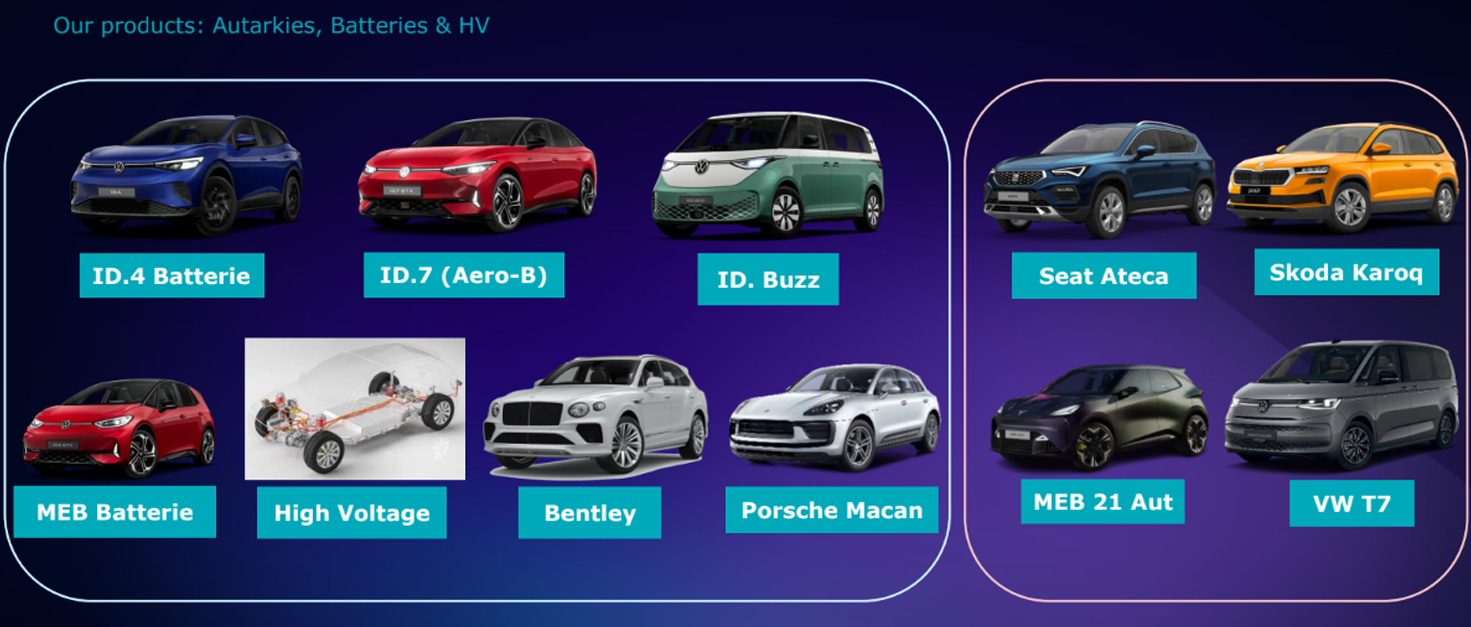
\includegraphics[width=0.9\linewidth]{images/Ch1/10.png}
        \caption{Les produits Autarkies, Batteries \& HV}
        \label{fig:produits_autarkies}
    \end{minipage}
\end{figure}

SEBN-MA est un fournisseur de premier rang (Tier 1) de l'industrie automobile, collaborant avec plusieurs constructeurs automobiles de renommée mondiale. Parmi ses principaux clients figurent les marques du groupe Volkswagen, telles que Volkswagen, Audi, Škoda, SEAT, CUPRA, Porsche et Bentley. Grâce à ses sites de production implantés au Maroc, l'entreprise assure l'approvisionnement des usines de ses clients situées principalement en Allemagne, en Espagne, en Slovaquie, en République tchèque et au Royaume-Uni, tout en garantissant des produits conformes aux exigences de qualité, de coût et de délai.

% ---------------------------------------------------------
% Note : LaTeX gérera automatiquement la numérotation. 
% Même si tu as écrit 1.5 dans ton brouillon, LaTeX l'affichera comme 1.4 car c'est la 4ème section.
\section{Organisation de l'entreprise}

\subsection{Principaux départements et leurs rôles}
L'efficacité industrielle du site repose sur une organisation fonctionnelle où chaque département contribue spécifiquement à la performance globale. Les principaux services et leurs missions sont décrits ci-après :

\begin{itemize}
    \item \textbf{Département Ressources Humaines (PHR) :} Le département RH a une double mission : il assure d'une part la gestion du volet administratif du personnel (la paie, les prestations sociales) et d'autre part la gestion de l'absentéisme et de la discipline.
    
    \item \textbf{Département Finance (PCP) :} Ce département a pour mission de gérer toutes les opérations de comptabilité et de trésorerie tout en restant en contact permanent avec les clients, les fournisseurs et les différents acteurs internes et externes à l'entreprise.
    
    \item \textbf{Département Controlling (PMC) :} Il coordonne, évalue et surveille toutes les activités liées au contrôle de gestion ainsi qu'aux opérations de suivi du budget.
    
    \item \textbf{Département Projet (PPM) :} Le département PO définit et maintient le référentiel des processus liés à la gestion de projet.
    
    \item \textbf{Département Technique (PTS) :} La principale mission de ce département (OHS-Environnement) est d'assurer l'application et la diffusion des règles de sécurité de l'entreprise en informant les employés sur les mesures de prévention. Il analyse les incidents afin d'en déterminer les causes et en déduit des actions d'amélioration et de prévention des risques.
    
    \item \textbf{Département Informatique (PIT) :} Chargé de l'administration du système d'information, le département informatique s'occupe de la gestion du parc informatique, incluant l'installation et l'entretien du réseau et des serveurs. En outre, ce service est chargé de gérer les applications et les ERP des différents départements.
    
    \item \textbf{Département Ingénierie (PPE) :} Ce département est chargé d'optimiser la planification de la production en fonction des besoins des clients et des objectifs internes. \textit{C'est le département dans lequel j'ai effectué mon stage.}
    
    \item \textbf{Département Production (PPR) :} La mission principale de ce département est d'assurer l'exécution de la production selon les normes des clients (fournies par le département planning) et selon les exigences des normes de qualité (normes client et normes IATF 16949).
    
    \item \textbf{Département Logistique (PLM) :} La fonction logistique a pour objectif de veiller à l'harmonie totale et à la parfaite synchronisation entre les flux de matières et les flux d'informations (production en Juste-à-Temps). Le département assure aussi l'approvisionnement, la gestion des stocks, l'ordonnancement de la production, le transport, etc.
\end{itemize}
\chapter{Contexte du Projet et Étude de l'Existant}
\label{chap:contexte_projet}

\section*{Introduction}
\addcontentsline{toc}{section}{Introduction}
Après avoir présenté l'entreprise SEBN-MA et son environnement industriel, ce chapitre est consacré au cadre spécifique de notre projet. Nous y détaillerons le fonctionnement des machines concernées, avant de présenter l'étude de l'existant concernant la gestion actuelle des indicateurs clés de performance (KPIs). Enfin, nous définirons la problématique soulevée, la solution web proposée et les indicateurs de succès du projet.

% ---------------------------------------------------------
\section{Cadre général du projet : Les machines HCM-S et CIM-3}
Ce projet cible particulièrement le suivi de production et l'analyse de performance d'un ensemble de machines spécifiques au sein de l'usine, désigné sous le terme de \textbf{« Set HCM-S / CIM-3 »}.

Pour comprendre l'enjeu du projet, il est essentiel de distinguer le rôle de ces deux types d'équipements :
\begin{itemize}
    \item \textbf{La machine HCM-S (Hyper Compact Machine - Set bar) :} C'est une machine de préparation qui se charge des opérations de coupe des câbles, de dénudage, de sertissage (\textit{crimping}) et de l'ajout des terminaux.
    \item \textbf{La machine CIM-3 (Computer Integrated Manufacturing) :} C'est la machine d'assemblage qui prend le relais pour effectuer l'insertion automatique des câbles préparés dans les connecteurs finaux.
\end{itemize}

\textbf{Le concept du « Set » :} La machine HCM-S possède une cadence de production environ trois fois plus rapide qu'une machine CIM-3. Ainsi, pour équilibrer la ligne de production et éviter les goulots d'étranglement, l'usine regroupe ces équipements sous forme de « Set » composé d'\textbf{une (1) machine HCM-S couplée à trois (3) machines CIM-3}. Le pilotage de la solution logicielle repose sur l'analyse des KPIs de ces ensembles synchronisés.

% ---------------------------------------------------------
\section{Étude de l'existant}
Dans le cadre de la gestion et du suivi des projets au sein de SEBN-MA, le pilotage de l'activité des Sets HCM-S / CIM-3 repose sur l'analyse rigoureuse d'indicateurs clés de performance. 

Actuellement, le processus de centralisation, de calcul et de mise en forme de ces données se déroule de la manière suivante :
\begin{enumerate}
    \item \textbf{Extraction des données brutes (\textit{Raw Data}) :} Les données de production sont extraites à l'aide d'un outil interne basé sur des macros Excel.
    \item \textbf{Génération manuelle des tableaux de bord :} À partir de ces données brutes, les superviseurs et responsables doivent construire manuellement les différents graphiques et tableaux de bord dans Excel.
    % \item \textbf{Restitution statique :} Une fois rédigés et mis en forme, les rapports générés sont statiques et figés.
\end{enumerate}

% ---------------------------------------------------------
\section{Critique de l'existant (Problématique)}
Bien que cet outil basé sur des macros Excel soit fonctionnel d'un point de vue calculatoire, il présente d'importantes limites opérationnelles :
\begin{itemize}
    \item \textbf{Tâches chronophages :} La création manuelle des tableaux de bord après l'extraction des données brutes constitue une perte de temps considérable sans valeur ajoutée directe.
    \item \textbf{Rapports statiques :} L'absence d'interactivité empêche une analyse dynamique et en profondeur (\textit{drill-down}) des baisses de performance.
    \item \textbf{Problèmes d'accessibilité et de collaboration :} Le fichier Excel limite la collaboration en temps réel et rend le partage des informations difficile entre les différentes parties prenantes, d'autant plus que l'outil est restreint au réseau interne de l'entreprise.
\end{itemize}

% ---------------------------------------------------------
\section{Objectifs du Projet et Solution proposée}
Face à ces limites, l'objectif principal de ce projet est de concevoir, développer et déployer une \textbf{application Web intuitive et sécurisée} permettant de piloter l'activité des projets HCM-S CIM3. La réalisation de cette solution s'articule autour de deux grandes finalités :

\subsection{Phase 1 : Moderniser et externaliser la restitution}
Il s'agit d'offrir une interface moderne, accessible à tout moment et depuis n'importe quel emplacement géographique. L'application permettra d'éditer, de visualiser de manière interactive les tableaux de bord KPI et de mettre en évidence les points marquants (\textit{highlights}) préalablement préparés.

\subsection{Phase 2 : Automatiser la chaîne de valeur}
L'objectif est d'éliminer définitivement les tâches chronophages en intégrant un moteur logiciel capable de lire et d'interpréter automatiquement les données issues de l'outil macro Excel, ou bien directement de la base de données centrale (et ce, malgré les restrictions du réseau interne). Ce moteur agira comme un ETL et générera de façon totalement automatisée les tableaux de bord directement sur l'application Web.

% ---------------------------------------------------------
\section{Indicateurs de succès du projet}
Pour valider l'aboutissement de notre application, plusieurs critères de succès stricts ont été définis avec l'entreprise d'accueil :
\begin{itemize}
    \item \textbf{Accessibilité continue :} Disponibilité 24h/24 et 7j/7 de l'application hors du réseau restreint de l'entreprise.
    \item \textbf{Confidentialité et sécurité :} Sécurisation stricte des accès pour les administrateurs via une authentification obligatoire et gestion rigoureuse des rôles utilisateurs.
    \item \textbf{Fiabilité des données :} Fidélité absolue des KPIs affichés sur l'application Web par rapport aux calculs initiaux.
\end{itemize}

\section*{Conclusion}
\addcontentsline{toc}{section}{Conclusion}
L'analyse de l'existant a mis en évidence le besoin crucial de moderniser le suivi des performances des équipements HCM-S et CIM-3. En passant d'un processus manuel sur Excel à une plateforme Web automatisée, SEBN-MA gagnera en réactivité et en fiabilité. Le chapitre suivant sera consacré à l'analyse détaillée des besoins de cette nouvelle application et à la conception de son architecture logicielle.
\chapter{Analyse et Spécification des Besoins}
\label{chap:analyse_besoins}

\section*{Introduction}
\addcontentsline{toc}{section}{Introduction}
Ce chapitre a pour objectif de détailler les exigences fonctionnelles et non fonctionnelles de la solution logicielle HCM-S CIM3. Nous y définirons les acteurs du système, leurs habilitations respectives, ainsi que les spécifications de l'application divisées en deux phases distinctes : la visualisation interactive (Phase 1) et l'automatisation de l'ingestion des données (Phase 2). Enfin, nous analyserons les défis techniques liés à l'infrastructure existante et proposerons des stratégies architecturales pour y répondre.

% ---------------------------------------------------------
\section{Acteurs et Rôles (User Roles)}
Contrairement à une application interne fermée, la solution mise en place prévoit une accessibilité publique pour la consultation, combinée à une gestion stricte des droits pour l'administration. Le système prévoit ainsi trois niveaux d'habilitation :

\begin{itemize}
    \item \textbf{Visiteur (User normal) :} Utilisateur grand public ou partie prenante n'ayant pas de compte. Il accède librement à l'application sans authentification. Ses droits sont strictement limités à la consultation (lecture seule) des tableaux de bord et des rapports. Il ne peut effectuer aucune altération de données.
    
    \item \textbf{Administrateur (Admin) :} Utilisateur authentifié responsable de l'alimentation quotidienne ou hebdomadaire de l'application. Ses prérogatives incluent :
    \begin{itemize}
        \item La création et gestion des projets HCM-S CIM3.
        \item La mise à jour des valeurs des KPIs.
        \item La rédaction et la publication des faits marquants (\textit{Highlights}).
        \item La gestion des clés d'API (création), sans possibilité d'accéder aux clés supprimées (\textit{soft deleted}).
        \item \textit{Restriction :} Il ne peut pas créer ni gérer les comptes d'autres administrateurs.
    \end{itemize}

    \item \textbf{Super Administrateur (Super Admin) :} L'acteur possédant les droits absolus sur l'application. En plus de toutes les prérogatives de l'Administrateur, il a l'autorité de créer, suspendre ou supprimer les comptes des autres Administrateurs et d'accéder aux données archivées (comme les API keys supprimées).
\end{itemize}

% ---------------------------------------------------------
\section{Spécifications Fonctionnelles (Requirements)}

\subsection{Exigences Communes et Sécurité}
\begin{itemize}
    \item \textbf{Authentification JWT :} L'accès aux espaces d'administration (Admin et Super Admin) sera sécurisé par une authentification par jeton (JSON Web Token).
    \item \textbf{Responsive Design :} Les interfaces graphiques doivent s'adapter de manière fluide et ergonomique aux écrans d'ordinateurs, ainsi qu'aux terminaux mobiles (Smartphones/Tablettes).
    \item \textbf{Disponibilité :} L'application doit être hébergée et accessible publiquement, garantissant une disponibilité continue (24h/24, 7j/7), indépendamment des pannes ou restrictions du réseau interne de l'entreprise.
\end{itemize}

\subsection{Exigences Phase 1 : Interface de Visualisation et d'Édition}
Durant cette première phase, l'application fonctionnera de manière autonome, alimentée manuellement par les administrateurs.

\begin{enumerate}
    \item \textbf{Module de Connexion :} Interface sécurisée (Email / Mot de passe) réservée aux Administrateurs et au Super Administrateur.
    
    \item \textbf{Espace d'Administration :}
    \begin{itemize}
        \item Interface de création et modification de projets (Nom, Date, Statut, affectation des Sets machines).
        \item Formulaire de saisie des KPIs avec possibilité d'importation en masse (\textit{Bulk Data Entry}) via un simple copier/coller depuis Excel.
        \item Éditeur de texte pour rédiger et formater les "Highlights" de chaque projet.
        \item Interface de gestion des accès (réservée au Super Admin).
        \item Gestionnaire de clés d'API (en préparation pour la Phase 2).
    \end{itemize}
    
    \item \textbf{Tableau de Bord interactif (Dashboard - Accès Public) :}
    \begin{itemize}
        \item Affichage dynamique des KPIs sous forme de graphiques interactifs.
        \item Menus de navigation pour basculer facilement d'un projet HCM-S CIM3 à un autre.
        \item Filtres par semaines pour la visualisation sur des périodes précises.
        \item Module comparatif permettant d'analyser l'évolution des KPIs d'une semaine à l'autre.
        \item Zone dédiée à la mise en évidence des "Highlights" rédigés par les administrateurs.
        \item Zone dédiée pour les "Key Takeaways" du project.
    \end{itemize}
\end{enumerate}

\subsection{Exigences Phase 2 : Automatisation de la Génération}
Cette phase vise à remplacer la saisie manuelle (Bulk Entry) par un flux de données automatisé.
\begin{itemize}
    \item \textbf{Intégration de l'outil métier :} Implémentation d'un module (API Endpoint) capable de recevoir directement les résultats issus de la macro Excel interne.
    \item \textbf{Extraction et parsing :} Le système devra extraire automatiquement les KPIs et les Highlights du \textit{payload} reçu et mettre à jour la base de données sans intervention humaine.
    \item \textbf{Historisation :} Sauvegarde systématique des états pour garantir la traçabilité et permettre les comparaisons temporelles prévues sur le Dashboard.
\end{itemize}

% ---------------------------------------------------------
\section{Défis Techniques et Stratégies d'Architecture}
Le déploiement de cette solution soulève d'importants défis d'intégration liés aux restrictions du réseau d'entreprise et à la gestion de la consistance des données. 

\subsection{Défi de Communication (Réseau Privé vs. Cloud)}
\textbf{Problématique :} L'outil générant les données brutes (Macro Excel) réside sur le réseau restreint de l'entreprise qui bloque les requêtes entrantes. L'application Web, hébergée sur le Cloud, ne peut donc pas "interroger" le fichier local. \\
\textbf{Stratégies à l'étude :}
\begin{itemize}
    \item \textit{Intégration VBA Directe (Push) :} Modification de la macro pour qu'elle exécute elle-même une requête HTTP POST sortante (sécurisée par une API Key) vers l'application Cloud après chaque mise à jour.
    \item \textit{Agent de synchronisation local :} Déploiement d'un script Python ou PowerShell en local, chargé d'envoyer quotidiennement les données vers l'API externe.
    \item \textit{Upload Asynchrone (Solution de repli) :} Export d'un fichier plat (JSON/Excel) par la macro, téléversé manuellement par l'administrateur via l'interface Web.
\end{itemize}

\subsection{Défi d'Ingestion des Données (Format d'Entrée)}
\textbf{Problématique :} Assurer une transition fluide et sans régression entre la saisie manuelle (Phase 1) et l'automatisation (Phase 2). \\
\textbf{Stratégie :} En Phase 1, l'insertion se fera via l'outil de \textit{Bulk Data Entry} ou des formulaires stricts. L'upload de documents statiques (PDF) est formellement exclu pour préserver l'interactivité. En Phase 2, l'ingestion basculera sur une API REST acceptant des \textit{payloads} JSON standardisés, avec une authentification par API Key.

\subsection{Défi de Granularité, Fidélité et Gestion du Temps}
\textbf{Problématique :} La pertinence des KPIs dépend de la finesse des données. Les périodes incomplètes (ex: milieu de semaine) risquent de fausser les moyennes. \\
\textbf{Stratégies à l'étude :}
\begin{itemize}
    \item \textit{Stockage de la donnée brute journalière :} Plutôt que d'envoyer des bilans figés, la macro exportera des données désagrégées. Le calcul des KPIs sera effectué dynamiquement par le Backend.
    \item \textit{Gestion du "Week-to-Date" :} Implémentation d'une logique Backend stricte pour différencier une "valeur nulle" (0\% de performance) d'une "absence de donnée", avec des indicateurs visuels signalant les périodes non clôturées.
\end{itemize}

\subsection{Défi du "Cold Start" et des Données Manquantes}
\textbf{Problématique :} Puisque l'application Cloud ne peut pas interroger la base locale à la volée, comment gérer les requêtes d'utilisateurs sur des dates non encore synchronisées, et comment fournir un historique au lancement de l'application ? \\
\textbf{Stratégie (Source de Vérité Unique) :}
\begin{itemize}
    \item La base de données PostgreSQL de l'application Web sera la seule source de vérité. L'interface limitera dynamiquement les sélecteurs de dates entre les valeurs \texttt{min\_date} et \texttt{max\_date} présentes en base, empêchant ainsi les requêtes dans le vide.
    \item Pour pallier le \textit{Cold Start} (base vide au lancement), une opération de \textit{Historical Backfill} sera réalisée : un export massif de tout l'historique disponible sera généré depuis Excel et injecté dans l'application. Cette injection respectera scrupuleusement la granularité journalière pour éviter les incohérences de calcul avec les futures données automatisées.
\end{itemize}

\section*{Conclusion}
\addcontentsline{toc}{section}{Conclusion}
L'analyse des besoins a permis de cartographier précisément les rôles des utilisateurs, les fonctionnalités attendues ainsi que les obstacles techniques inhérents à l'infrastructure réseau de SEBN-MA. Ces spécifications servent de fondation solide pour la phase suivante, dédiée à la conception architecturale de la solution, où nous traduirons ces besoins en modèles techniques et en diagrammes UML.
\chapter{Architecture et Conception du Système}
\label{chap:architecture_conception}

\section*{Introduction}
\addcontentsline{toc}{section}{Introduction}
Suite à l'analyse détaillée des besoins, ce chapitre est consacré à la conception technique de la solution. Nous y présenterons l'architecture globale de l'application, les choix technologiques adoptés, ainsi que la modélisation statique (diagramme de classes) et dynamique (diagrammes de séquence) du système. Enfin, nous détaillerons les mécanismes de sécurité mis en place pour garantir l'intégrité des données industrielles.

% ---------------------------------------------------------
\section{Architecture Globale et Choix Technologiques}

\subsection{Pattern d'Architecture}
L'application repose sur une architecture découplée de type \textbf{Client/Serveur} (Single Page Application + API REST).
Le backend adopte une architecture en couches inspirée du \textbf{Domain-Driven Design (DDD)}, séparant strictement la logique de présentation (API/Routes), la logique métier (Services) et l'accès aux données (Modèles). Le frontend, quant à lui, est structuré par fonctionnalités (\textit{Feature-Driven Component-Based}).

\begin{figure}[H]
    \centering
    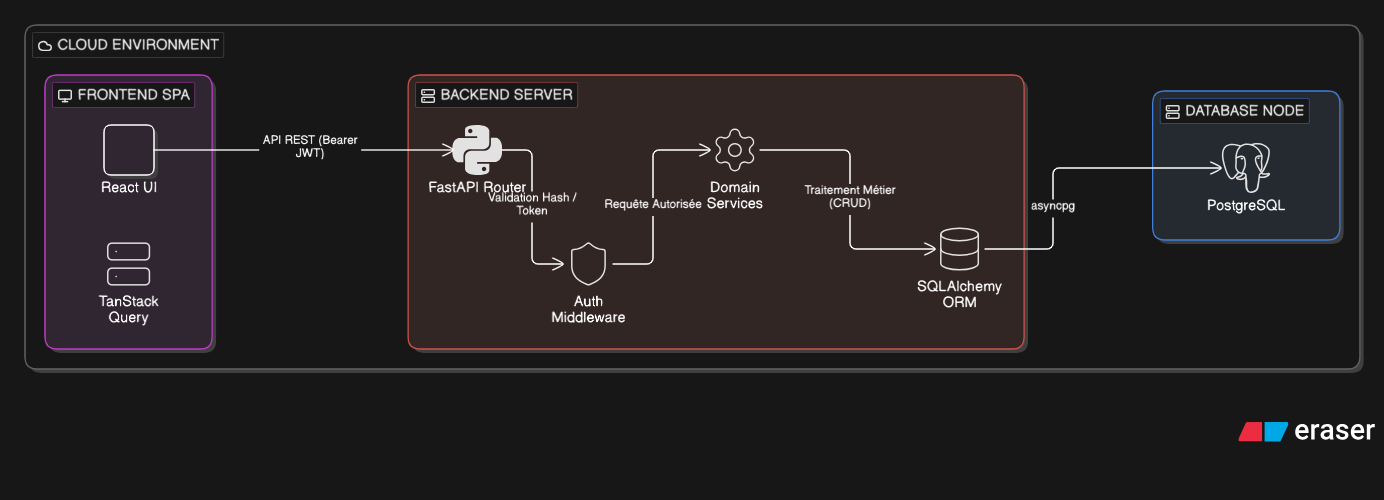
\includegraphics[width=0.8\textwidth]{images/ch4/arch.png}
    \caption{Architecture globale et flux de communication du système}
    \label{fig:architecture_globale}
\end{figure}

\subsection{Stack Technologique}
Pour répondre aux exigences de performance et de modernité, les technologies suivantes ont été retenues :

\begin{itemize}
    \item \textbf{Frontend (Client Web) :} 
    \begin{itemize}
        \item \textbf{React 19 (TypeScript) / Vite :} Pour un typage statique strict et un rendu réactif.
        \item \textbf{Tailwind CSS v4 :} Pour un design système rapide et responsive.
        \item \textbf{TanStack Query :} Pour la mise en cache intelligente et la gestion asynchrone des requêtes.
        \item \textbf{Chart.js :} Pour la visualisation dynamique des tendances des KPIs.
    \end{itemize}
    
    \item \textbf{Backend (API REST) :}
    \begin{itemize}
        \item \textbf{Python (FastAPI) :} Choisi pour ses hautes performances (asynchrone natif) et sa génération automatique de documentation (Swagger/OpenAPI).
        \item \textbf{SQLAlchemy 2.0 \& Pydantic v2 :} Pour le mapping objet-relationnel (ORM) asynchrone et la validation stricte des flux d'entrée/sortie.
    \end{itemize}
    
    \item \textbf{Base de données :} 
    \begin{itemize}
        \item \textbf{PostgreSQL :} Déployé via le driver asynchrone \texttt{asyncpg}, garantissant robustesse et intégrité relationnelle.
    \end{itemize}
\end{itemize}

\subsection{Étude Comparative et Justification des Choix (Benchmark)}
Le choix d'une architecture découplée \textbf{FastAPI (Backend) + React SPA (Frontend)} face à un framework full-stack unifié tel que \textbf{Next.js} (Node.js) a été guidé par les contraintes spécifiques du contexte industriel de SEBN-MA. Le tableau~\ref{tab:benchmark_archi} résume cette analyse comparative.

\begin{table}[H]
\centering
\small
\renewcommand{\arraystretch}{1.3}
\begin{tabular}{|p{3.8cm}|p{5.5cm}|p{5.5cm}|}
\hline
\textbf{Critère d'évaluation} & \textbf{Next.js (Monolithe Full-Stack Node.js)} & \textbf{Solution Retenue : FastAPI + React SPA} \\
\hline
\hline
\textbf{Nature de l'application \& Référencement (SEO)} & Conçu pour le rendu côté serveur (SSR) et le SEO public (e-commerce, vitrines). & Application intranet métier dédiée. Le SSR est inutile ; une SPA client-side servie statiquement offre une fluidité maximale. \\
\hline
\textbf{Écosystème Data \& Calculs Industriels} & Écosystème JavaScript limité pour l'analyse mathématique et statistique avancée. & Écosystème Python incontournable (NumPy, Pandas, SciPy), ouvrant la voie à la maintenance prédictive et au Machine Learning. \\
\hline
\textbf{Interopérabilité \& API First} & Logique serveur souvent couplée aux Server Actions et composants React. & API REST pure, documentée nativement (\textit{OpenAPI/Swagger}), facilement consommable par des scripts Python et macros Excel. \\
\hline
\textbf{Performances d'ingestion (I/O intensives)} & Bonnes performances en I/O, mais ORMs Node.js (ex: Prisma) plus lourds en écriture de masse. & Moteur asynchrone (\textit{Starlette + Pydantic v2} en Rust) avec driver \texttt{asyncpg}, offrant un débit exceptionnel en \textit{Bulk Insert}. \\
\hline
\textbf{Déploiement en milieu industriel (On-Premise)} & Nécessite un runtime Node.js permanent ou des fonctions Serverless (ex: Vercel). & Découplage total : API conteneurisée (Docker léger) et Frontend compilable en fichiers statiques (Nginx/CDN). \\
\hline
\end{tabular}
\caption{Comparatif architectural : Next.js versus FastAPI / React SPA}
\label{tab:benchmark_archi}
\end{table}

Cette analyse met en lumière trois arguments décisifs en faveur de la solution retenue :
\begin{enumerate}
    \item \textbf{La vocation multi-clients de l'API (Approche API-First) :} L'application ne s'adresse pas uniquement aux navigateurs web. La phase 2 du projet requiert l'ingestion automatique de données issues de macros Excel et de scripts d'automatisation. FastAPI permet d'exposer une API REST découplée, standardisée, validée par Pydantic et sécurisée par clés d'API, indépendamment du cycle de vie de l'interface graphique.
    \item \textbf{La synergie avec le traitement de données industrielles :} Python constitue la référence absolue pour le traitement des séries temporelles et le calcul des métriques de production (OEE, Scrap Rate, CIM). L'utilisation de FastAPI garantit une intégration naturelle avec les futures briques d'intelligence artificielle et d'analyse prédictive envisagées par l'usine.
    \item \textbf{L'absence de besoin en rendu serveur (SSR) :} Les tableaux de bord de supervision interne ne nécessitent aucun référencement naturel. L'utilisation d'une Single Page Application (SPA) propulsée par React 19 et \textit{TanStack Query} élimine la charge serveur liée au SSR, tout en assurant une mise en cache locale instantanée pour les utilisateurs sur les lignes de production.
\end{enumerate}

% ---------------------------------------------------------
\section{Modélisation de la Base de Données}
La structuration des données est le cœur de notre application. Elle doit permettre de relier efficacement les équipements (machines HCM-S et CIM-3) à leurs indicateurs de performance, tout en conservant une traçabilité totale.

\begin{figure}[H]
    \centering
    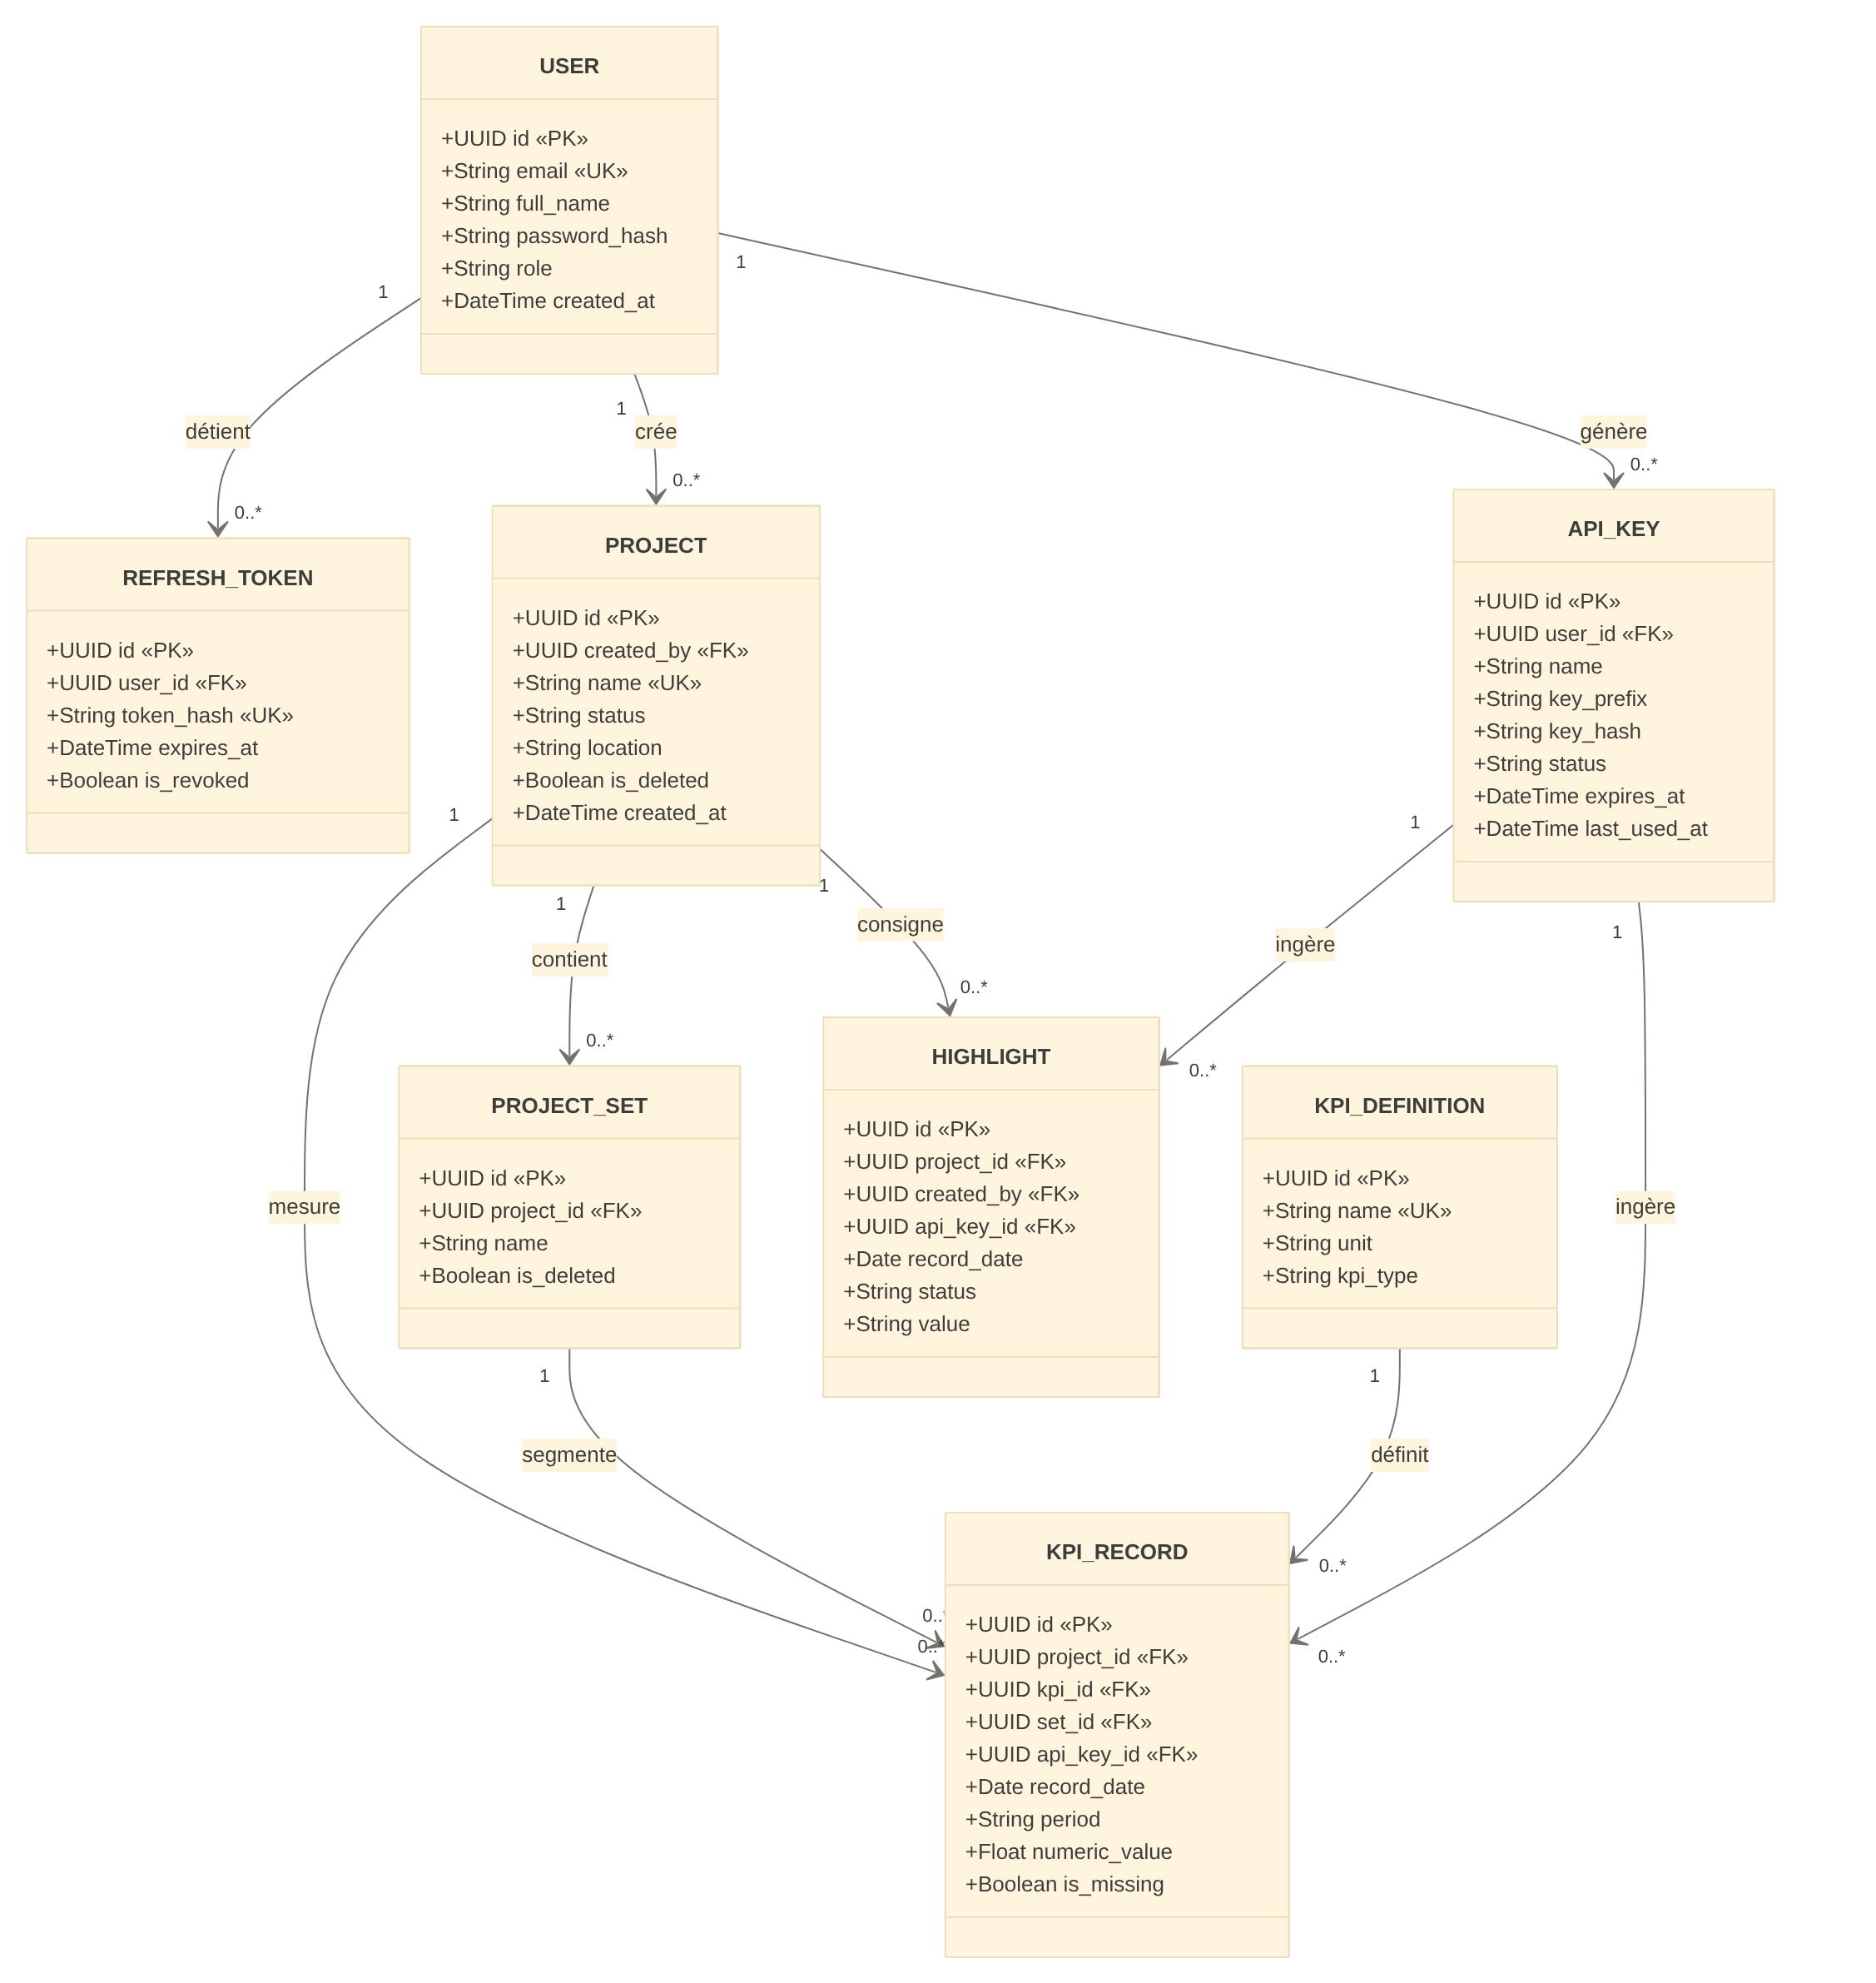
\includegraphics[width=0.9\textwidth]{images/ch4/uml_class.png}
    \caption{Diagramme de classes UML}
    \label{fig:diagramme_classes}
\end{figure}

\subsection{Entités Principales}
Le modèle relationnel s'articule autour de deux axes majeurs :
\begin{enumerate}
    \item \textbf{Axe Structurel et Sécurité :}
    \begin{itemize}
        \item \textbf{User :} Gère les administrateurs avec leurs rôles (Admin, Super Admin).
        \item \textbf{ApiKey :} Stocke les clés d'ingestion automatisées pour la Phase 2.
    \end{itemize}
    \item \textbf{Axe Métier (Industriel) :}
    \begin{itemize}
        \item \textbf{Project \& ProjectSet :} Représentent les lignes de production et leurs sous-ensembles machines (le "Set" HCM-S / CIM-3).
        \item \textbf{KPIDefinition :} Le référentiel des métriques mesurées (ex: TRS, Absentéisme, Qualité) avec leurs unités.
        \item \textbf{KPIRecord \& Highlight :} Les valeurs réelles mesurées dans le temps et les faits marquants associés.
    \end{itemize}
\end{enumerate}

\subsection{Stratégie de "Soft Delete" et Intégrité}
Dans un contexte industriel, la perte de données statistiques est inacceptable. C'est pourquoi une stratégie de suppression logique (\textit{Soft Delete}) a été implémentée :
\begin{itemize}
    \item \textbf{Drapeau Booléen :} Les projets et sets de machines ne sont jamais détruits physiquement de la base. Un attribut \texttt{is\_deleted = True} les masque des requêtes courantes, préservant ainsi l'historique des KPIs associés.
    \item \textbf{Machine à états pour les clés API :} Une clé passe de \textit{ACTIVE} à \textit{REVOKED} puis \textit{DELETED}. La clé est conservée pour garantir l'auditabilité des enregistrements (\texttt{api\_key\_id}) ayant été ingérés dans le passé.
\end{itemize}

% ---------------------------------------------------------
\section{Sécurité et Gestion des Accès}
La plateforme HCM-S CIM3 expose des données sensibles et nécessite une gestion stricte des identités, répartie en trois niveaux (Visiteur, Admin, Super Admin).

\subsection{Authentification des utilisateurs (JWT)}
Les accès humains sont gérés via le standard JSON Web Token (JWT) avec un motif à double jeton (\textit{Double Token Pattern}) :
\begin{itemize}
    \item Un \textbf{Access Token} de courte durée (utilisé pour les requêtes API).
    \item Un \textbf{Refresh Token} de longue durée, stocké sous forme de condensat (hash) en base, permettant de renouveler la session de manière transparente grâce à des intercepteurs \texttt{Axios} côté Frontend.
\end{itemize}

\subsection{Sécurisation de l'Ingestion (API Keys)}
Pour la Phase 2 (l'automatisation par script), l'authentification s'effectue via des clés d'API. Le backend applique le principe de \textit{Zero-Knowledge Storage} :
La clé générée n'est affichée qu'une seule fois à l'utilisateur. Seul un condensat cryptographique fort (\textbf{SHA-256}) est stocké en base de données. Lors d'une requête, le backend recalcule le hash du jeton reçu et le compare à celui stocké, garantissant qu'une compromission de la base de données ne révèle pas les clés d'accès.

% ---------------------------------------------------------
\section{Conception Dynamique : Diagrammes de Séquence}
Pour illustrer le comportement dynamique du système, nous avons modélisé les deux processus critiques du cycle de vie de la donnée : son ingestion et sa restitution.

\subsection{Phase 1 : Ingestion Automatisée des KPIs}
Le flux suivant décrit l'action du script externe poussant les données de la Macro Excel vers l'API.

\begin{figure}[H]
    \centering
    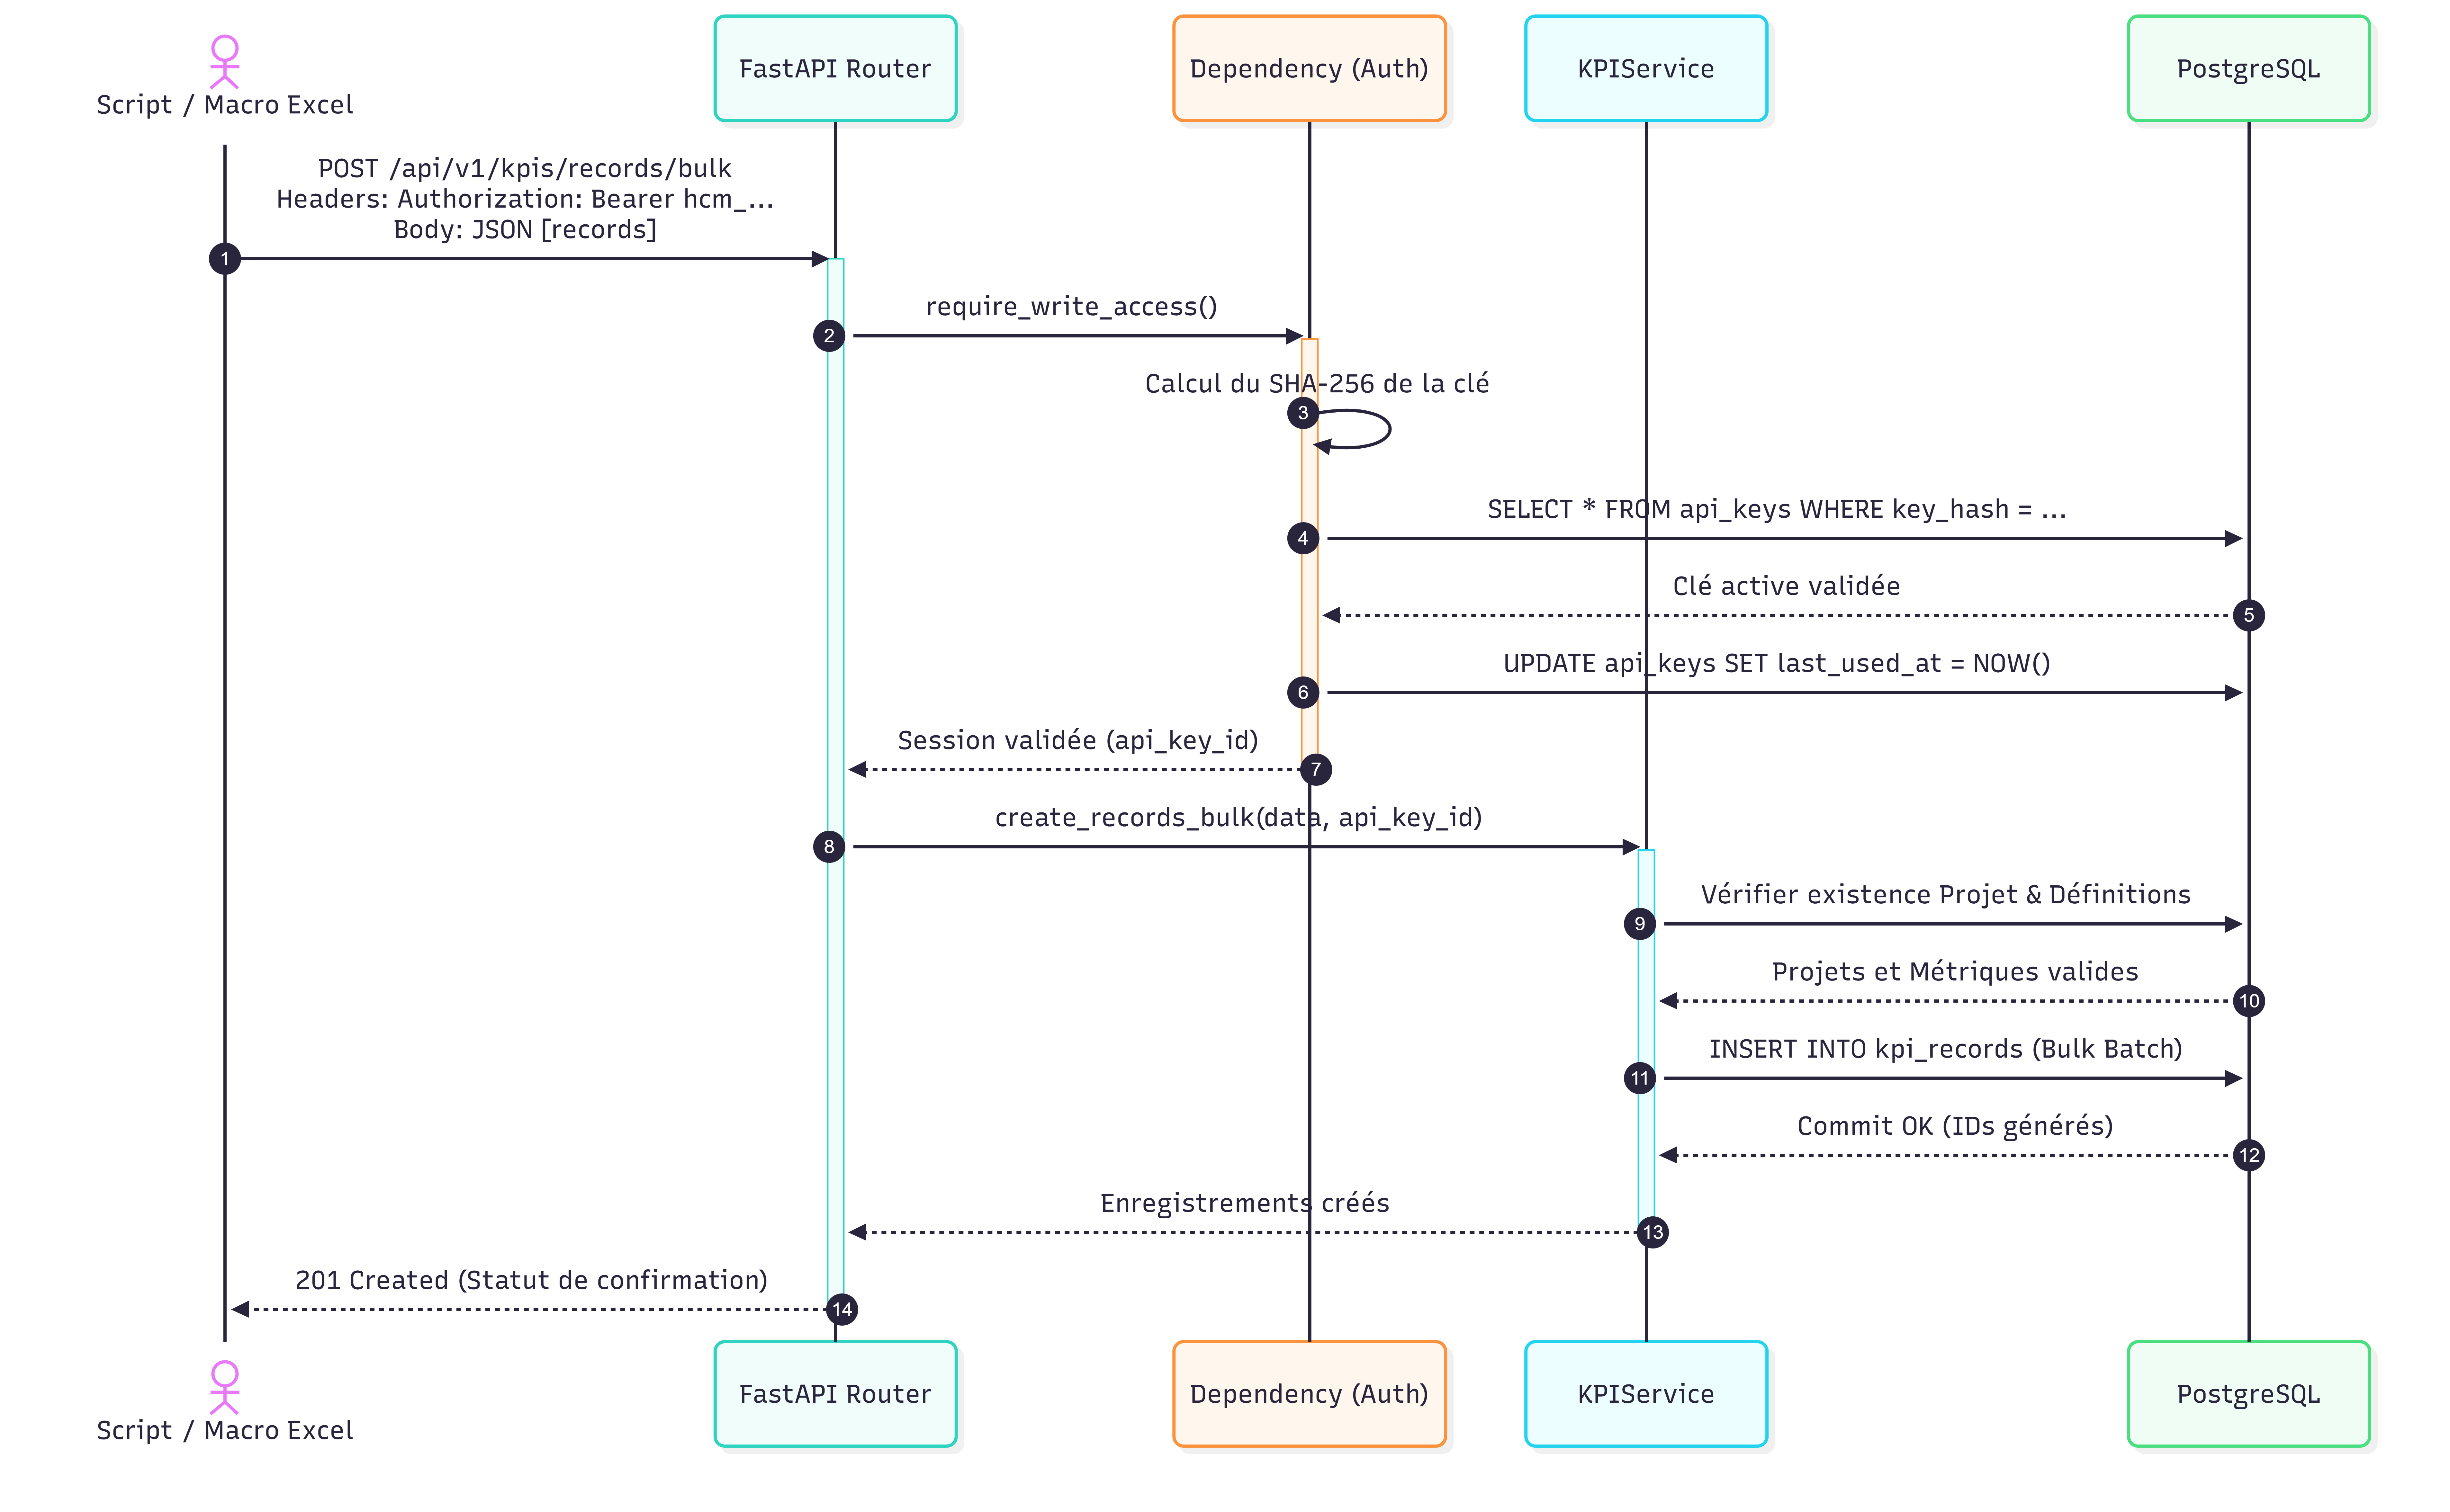
\includegraphics[width=0.85\textwidth]{images/ch4/sequence.png}
    \caption{Diagramme de séquence : Ingestion des données via API Key}
    \label{fig:seq_ingestion}
\end{figure}

\textbf{Description du flux :}
\begin{enumerate}
    \item Le script externe émet une requête \texttt{POST} contenant le payload JSON des KPIs, accompagnée de l'API Key dans l'en-tête \texttt{Authorization}.
    \item Le backend intercepte la requête, hache la clé et vérifie sa validité (statut actif, non expirée).
    \item Le service métier valide l'intégrité des données (existence du projet cible, types de valeurs).
    \item Les enregistrements sont insérés en lot (\textit{Bulk Insert}) de manière asynchrone dans PostgreSQL, et un code 201 (Created) est retourné.
\end{enumerate}

\subsection{Phase 2 : Restitution et Tableau de Bord}
Ce second flux illustre la récupération et la transformation des données lorsqu'un utilisateur (Manager) consulte le Dashboard.

\begin{figure}[H]
    \centering
    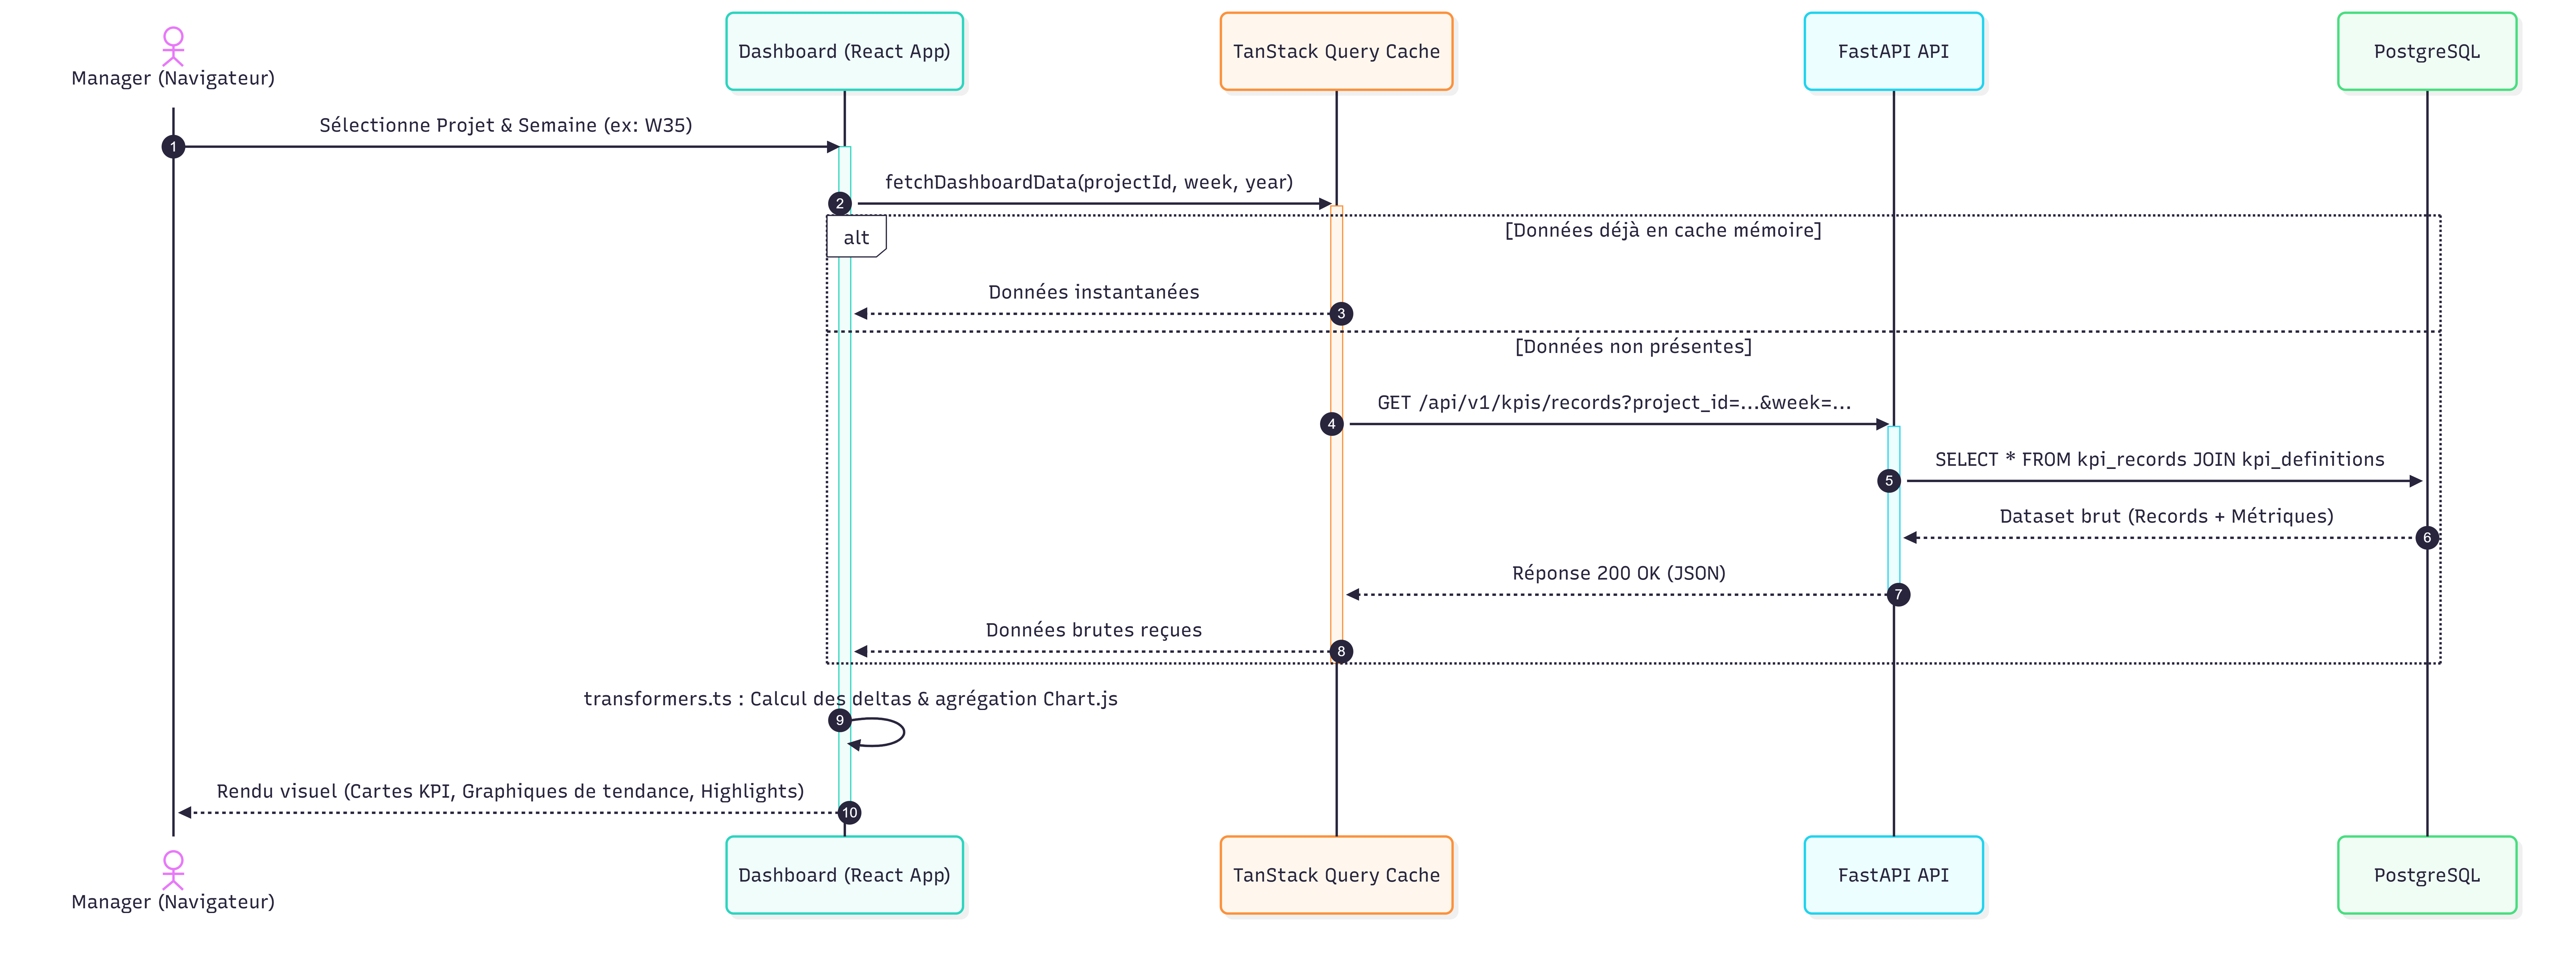
\includegraphics[width=0.85\textwidth]{images/ch4/seq_dashboard.png}
    \caption{Diagramme de séquence : Consultation du Dashboard}
    \label{fig:seq_dashboard}
\end{figure}

\textbf{Description du flux :}
\begin{enumerate}
    \item L'utilisateur sélectionne un projet et une période temporelle sur le Frontend.
    \item Le hook React (propulsé par TanStack Query) déclenche une requête \texttt{GET} vers le Backend.
    \item L'API interroge la base de données via l'ORM en effectuant une jointure optimisée entre les enregistrements (\texttt{KPIRecord}) et leurs définitions (\texttt{KPIDefinition}).
    \item Le Frontend reçoit le dataset brut. Un module de transformation côté client agrège les données, calcule les écarts différentiels (Deltas) et formate les séries chronologiques pour le rendu final dans les composants graphiques (\texttt{Chart.js}).
\end{enumerate}

\section*{Conclusion}
\addcontentsline{toc}{section}{Conclusion}
Les choix architecturaux et la modélisation retenus permettent de répondre efficacement aux problématiques identifiées. Le découplage des composants, associé à une modélisation robuste (Soft Delete) et une sécurité renforcée (Zero-Knowledge, JWT), assure la pérennité du système. Le chapitre suivant sera consacré à la réalisation concrète de cette architecture et à la présentation des interfaces finales.
\chapter{Réalisation et Implémentation}
\label{chap:realisation}

\section*{Introduction}
\addcontentsline{toc}{section}{Introduction}
Après avoir défini l'architecture théorique du système, ce dernier chapitre est consacré à la réalisation du projet. Nous y détaillerons l'environnement de développement, les choix d'implémentation spécifiques côté Backend et Frontend, ainsi que les stratégies de sécurité appliquées. Enfin, nous présenterons le résultat final à travers une cartographie des interfaces graphiques de l'application.

% ---------------------------------------------------------
\section{Environnement de Développement et DevOps}
Pour garantir la robustesse et la maintenabilité du code, l'environnement de développement a été standardisé autour d'outils modernes :

\begin{itemize}
    \item \textbf{Gestionnaires de paquets :} Utilisation de \textbf{npm} pour le Frontend (Node.js) et de \textbf{uv} (un gestionnaire ultra-rapide écrit en Rust) pour la résolution déterministe des dépendances Python du Backend.
    \item \textbf{Qualité du code (Linting) :} L'analyse statique du code Frontend est assurée par \textbf{Oxlint} et le compilateur \textbf{TypeScript} (\texttt{tsc}), garantissant l'absence d'erreurs de typage avant la compilation.
    \item \textbf{Conteneurisation (Docker) :} Le Backend et la base de données PostgreSQL sont conteneurisés via \texttt{docker-compose}. L'image de l'API est construite via un \textit{Multi-stage build} afin de minimiser le poids final et de réduire la surface d'attaque.
    \item \textbf{Intégration Continue (CI/CD) :} Un pipeline automatisé sur \textbf{GitHub Actions} exécute les tests unitaires à chaque modification du code et déploie automatiquement l'image sur Docker Hub lors d'une fusion sur la branche principale.
\end{itemize}

% ---------------------------------------------------------
\section{Implémentation du Backend (FastAPI)}

\subsection{Ingestion des Données et ORM Asynchrone}
La couche d'accès aux données de l'API a été développée de manière 100\% asynchrone (non-bloquante) grâce à \textbf{SQLAlchemy 2.0} et au driver \texttt{asyncpg}. 
Le processus d'ingestion en masse (\textit{Bulk Entry}) valide chaque ligne de KPI (type de donnée, existence du projet), attache automatiquement l'auteur de la modification (Administrateur ou Clé d'API), et insère les données de manière atomique (une seule transaction SQL) pour garantir l'intégrité de la base.

\subsection{Sécurité et Hachage Cryptographique}
La protection des données et des accès repose sur le module natif Python \texttt{hashlib} :
\begin{itemize}
    \item \textbf{Mots de passe Utilisateurs :} Hachés selon le standard industriel \textbf{PBKDF2-HMAC-SHA256} avec l'ajout d'un sel cryptographique aléatoire et 100 000 itérations, rendant les attaques par force brute inefficaces.
    \item \textbf{Clés d'API (Principe du \textit{Zero-Knowledge}) :} Lors de la génération d'une clé d'API pour la macro Excel/Script Python, celle-ci n'est affichée qu'une seule fois. Seul un condensat \textbf{SHA-256} est stocké en base de données.
\end{itemize}

% ---------------------------------------------------------
\section{Implémentation du Frontend (React)}

\subsection{Gestion d'état et Cache Serveur}
Plutôt que d'utiliser des états locaux complexes, l'application exploite \textbf{TanStack Query} pour gérer le cache serveur. Les données du Dashboard sont mises en cache de manière intelligente. Cela permet de minimiser les appels à l'API et d'offrir une interface extrêmement réactive lors du changement de filtres temporels.

\subsection{Rafraîchissement Silencieux du Token (Intercepteur Axios)}
Pour offrir une expérience utilisateur fluide (sans déconnexions soudaines), un intercepteur réseau a été développé avec \textbf{Axios} :
Lorsqu'une requête API échoue à cause d'un \textit{Access Token} expiré (Erreur 401), l'intercepteur suspend la requête, utilise le \textit{Refresh Token} en arrière-plan pour obtenir de nouveaux identifiants, met à jour le cache local, puis rejoue la requête initiale de manière totalement transparente pour l'utilisateur.

\subsection{Interface Utilisateur (UI/UX)}
L'interface a été conçue sur mesure à l'aide de \textbf{Tailwind CSS v4}, permettant un \textit{Responsive Design} parfait sans surcharger l'application avec des bibliothèques de composants lourdes. Les graphiques dynamiques sont propulsés par \textbf{Chart.js}, offrant des visualisations claires des tendances hebdomadaires.

% ---------------------------------------------------------
\section{Présentation des Interfaces de l'Application}
Cette section illustre le résultat final du projet à travers les écrans clés de la plateforme HCM-S CIM3.

\subsection{Espace Public et Consultation}

\begin{figure}[H]
    \centering
    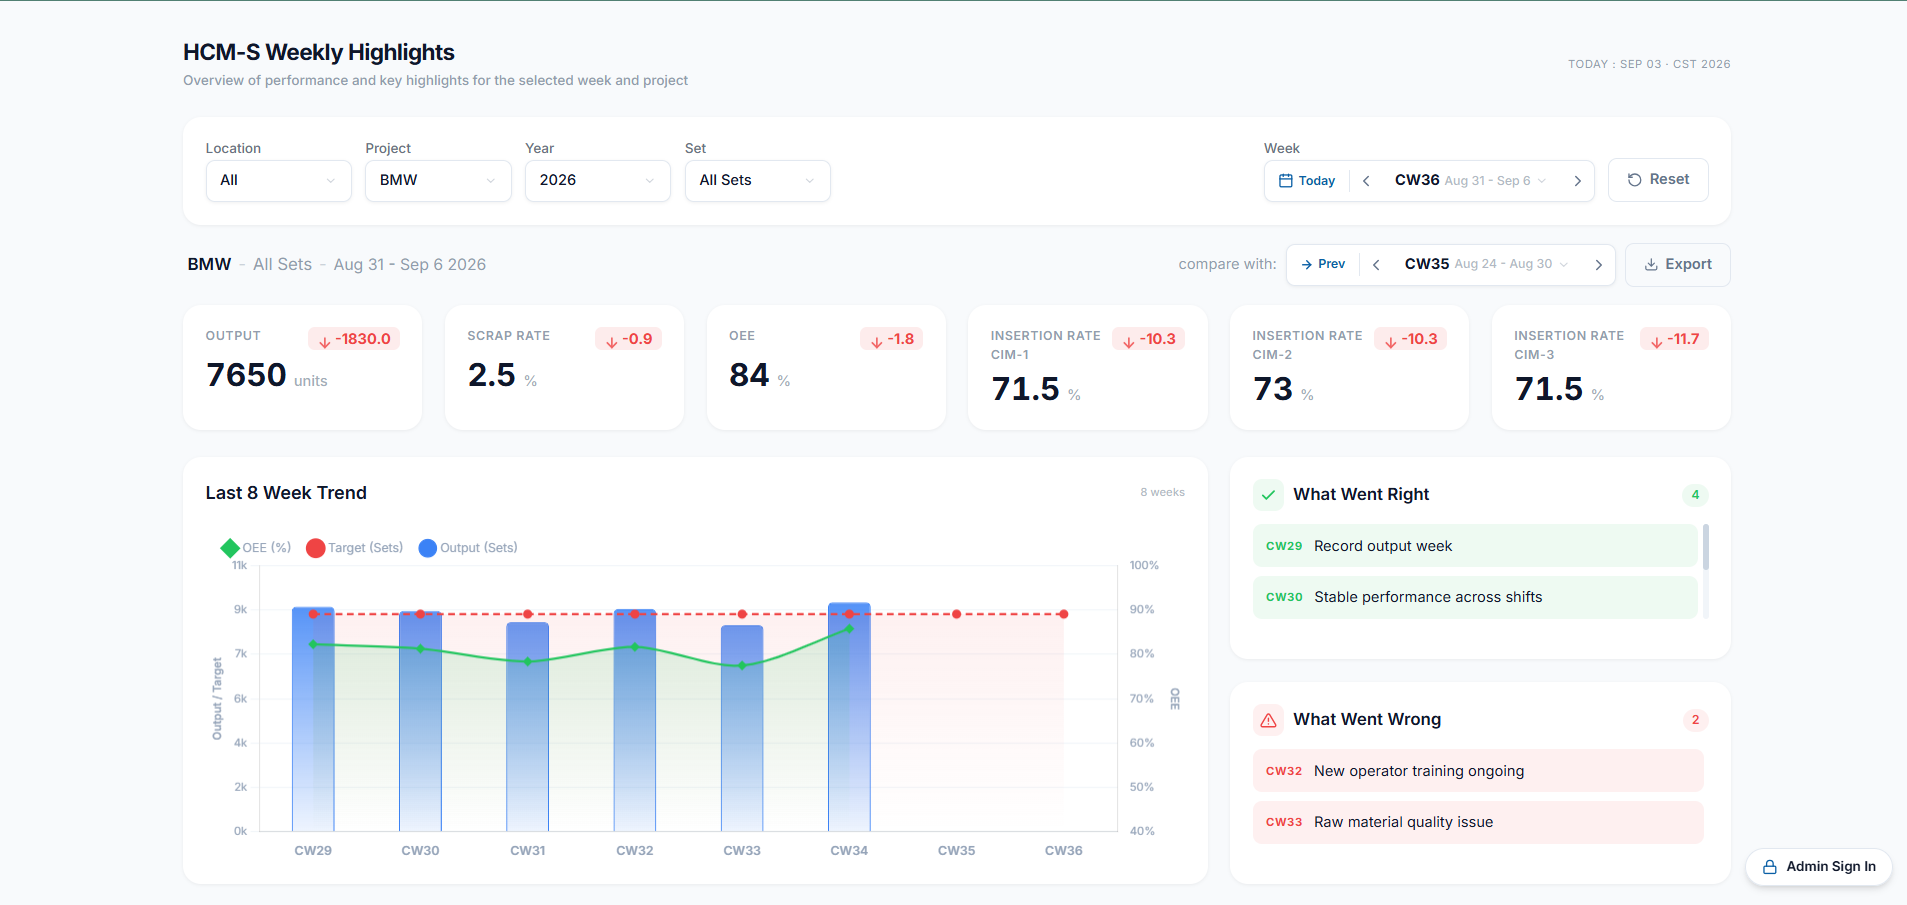
\includegraphics[width=0.9\textwidth]{images/Ch5/dashboard.png}
    \caption{Tableau de bord (Dashboard) interactif : Suivi des performances et tendances}
    \label{fig:ui_dashboard}
\end{figure}

Le tableau de bord permet de filtrer les données par Projet, Set de machines, Année et Semaine. Il affiche les deltas comparatifs et génère des graphiques d'évolution grâce au module de transformation intégré au Frontend.

\subsection{Espaces d'Administration et Saisie}

\begin{figure}[H]
    \centering
    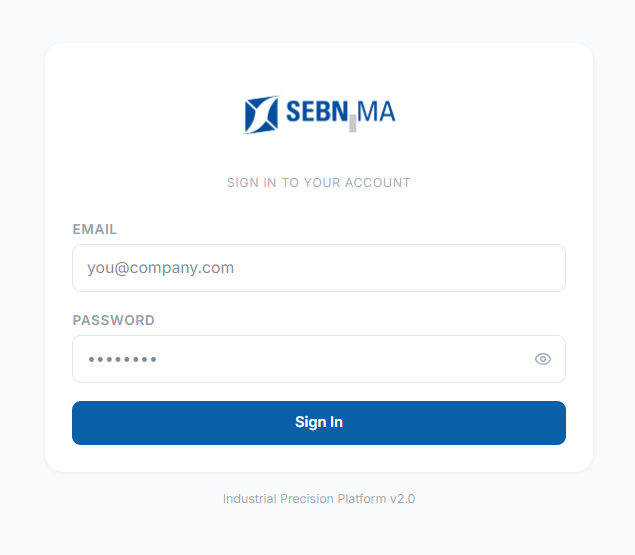
\includegraphics[width=0.6\textwidth]{images/Ch5/login.png}
    \caption{Portail d'authentification sécurisé}
    \label{fig:ui_login}
\end{figure}

\begin{figure}[H]
    \centering
    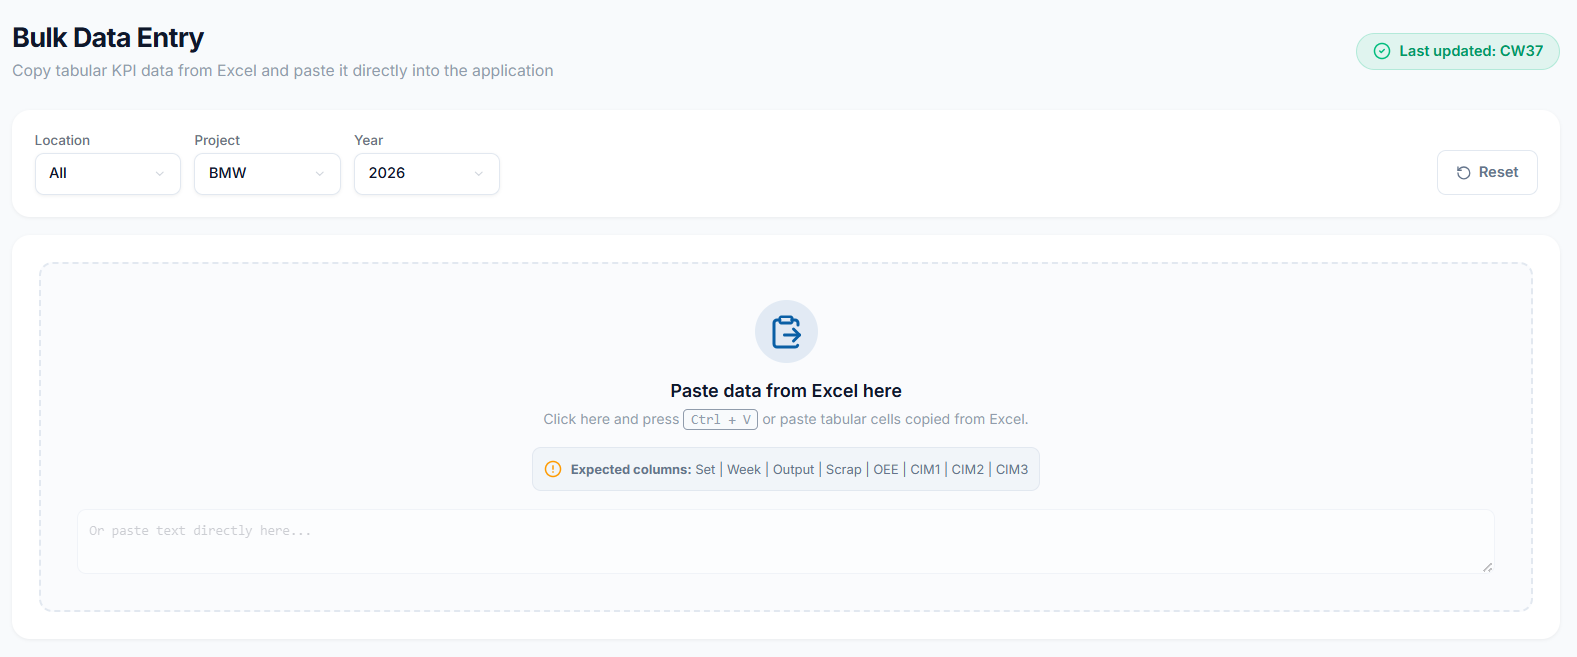
\includegraphics[width=0.9\textwidth]{images/Ch5/bulk.png}
    \caption{Interface de saisie en masse (Bulk Data Entry) avec parsing du presse-papiers Excel}
    \label{fig:ui_bulk_entry}
\end{figure}

\begin{figure}[H]
    \centering
    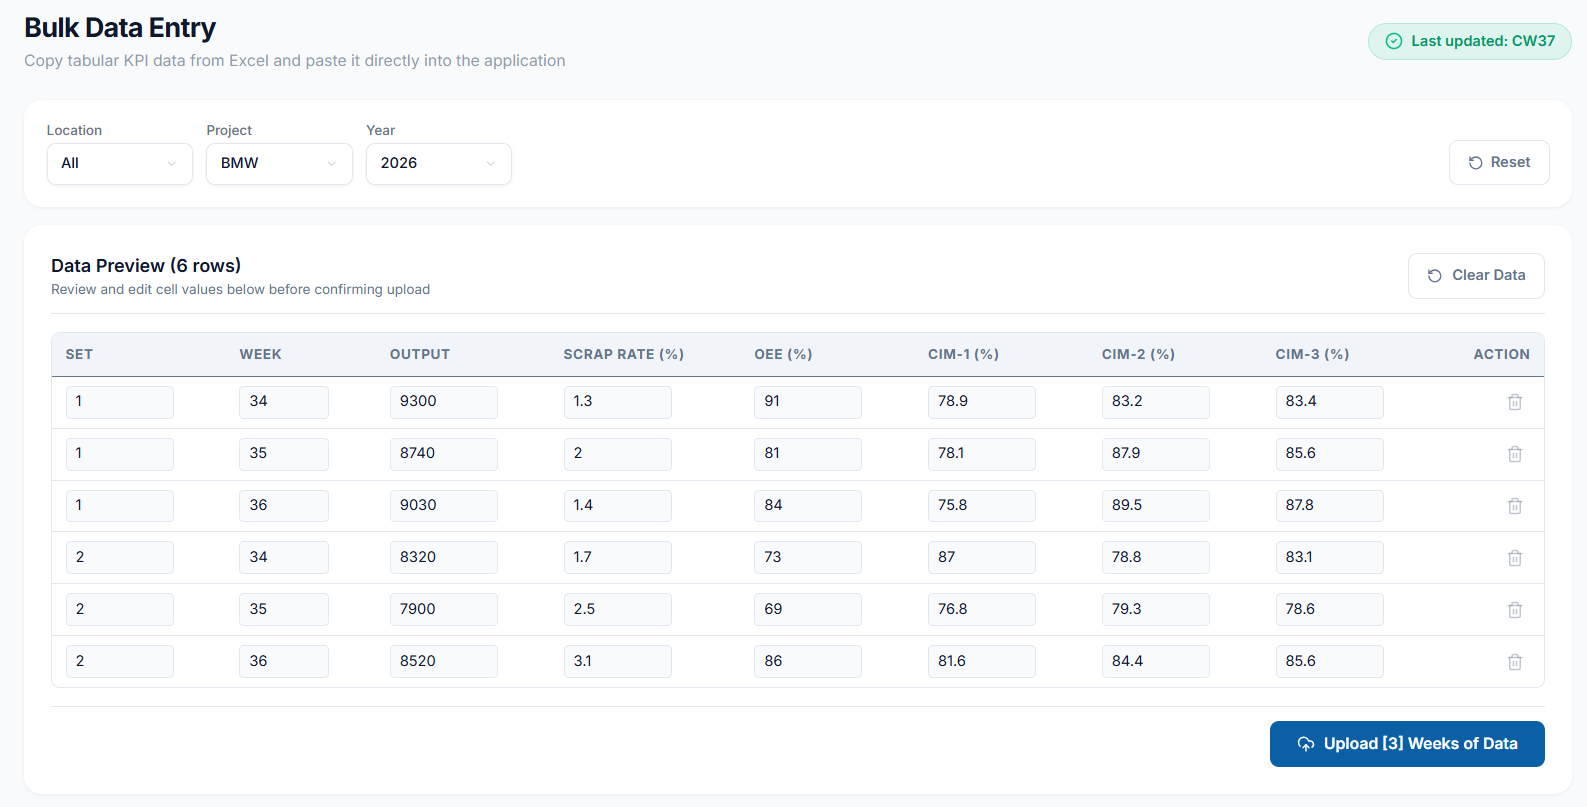
\includegraphics[width=0.9\textwidth]{images/Ch5/bulk_data.png}
    \caption{Interface de saisie en masse (Bulk Data Entry) après l'insertion des données}
    \label{fig:ui_bulk_entry_with_data}
\end{figure}

L'interface de saisie en masse a été conçue pour faciliter la transition des utilisateurs. Elle permet de copier directement les données depuis l'ancien outil Excel et de les coller dans l'application, qui valide automatiquement les formats et les numéros de semaines avant l'envoi au serveur.

\subsection{Gestion du Système (Super Admin)}

% Affichage de deux images côte à côte pour gagner de l'espace
\begin{figure}[H]
    \centering
    \begin{minipage}{0.48\textwidth}
        \centering
        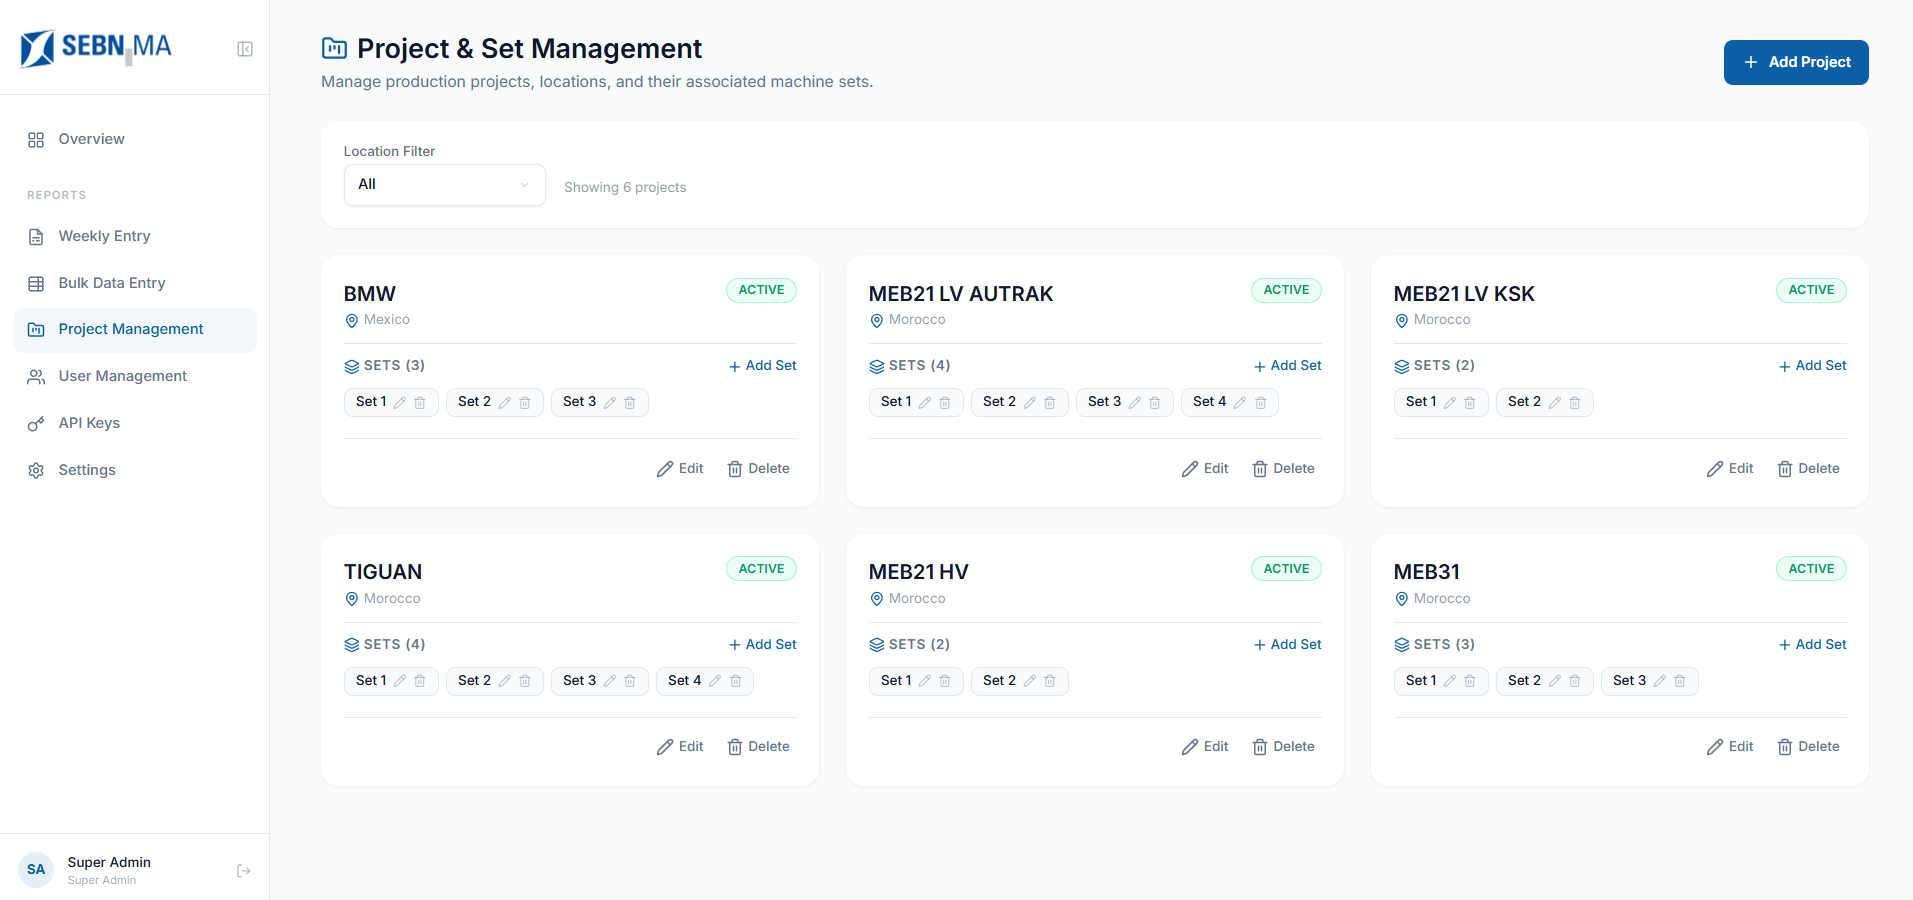
\includegraphics[width=\linewidth]{images/Ch5/projects.png}
        \caption{Gestion des Projets et des Sets machines}
        \label{fig:ui_projects}
    \end{minipage}\hfill
    \begin{minipage}{0.48\textwidth}
        \centering
        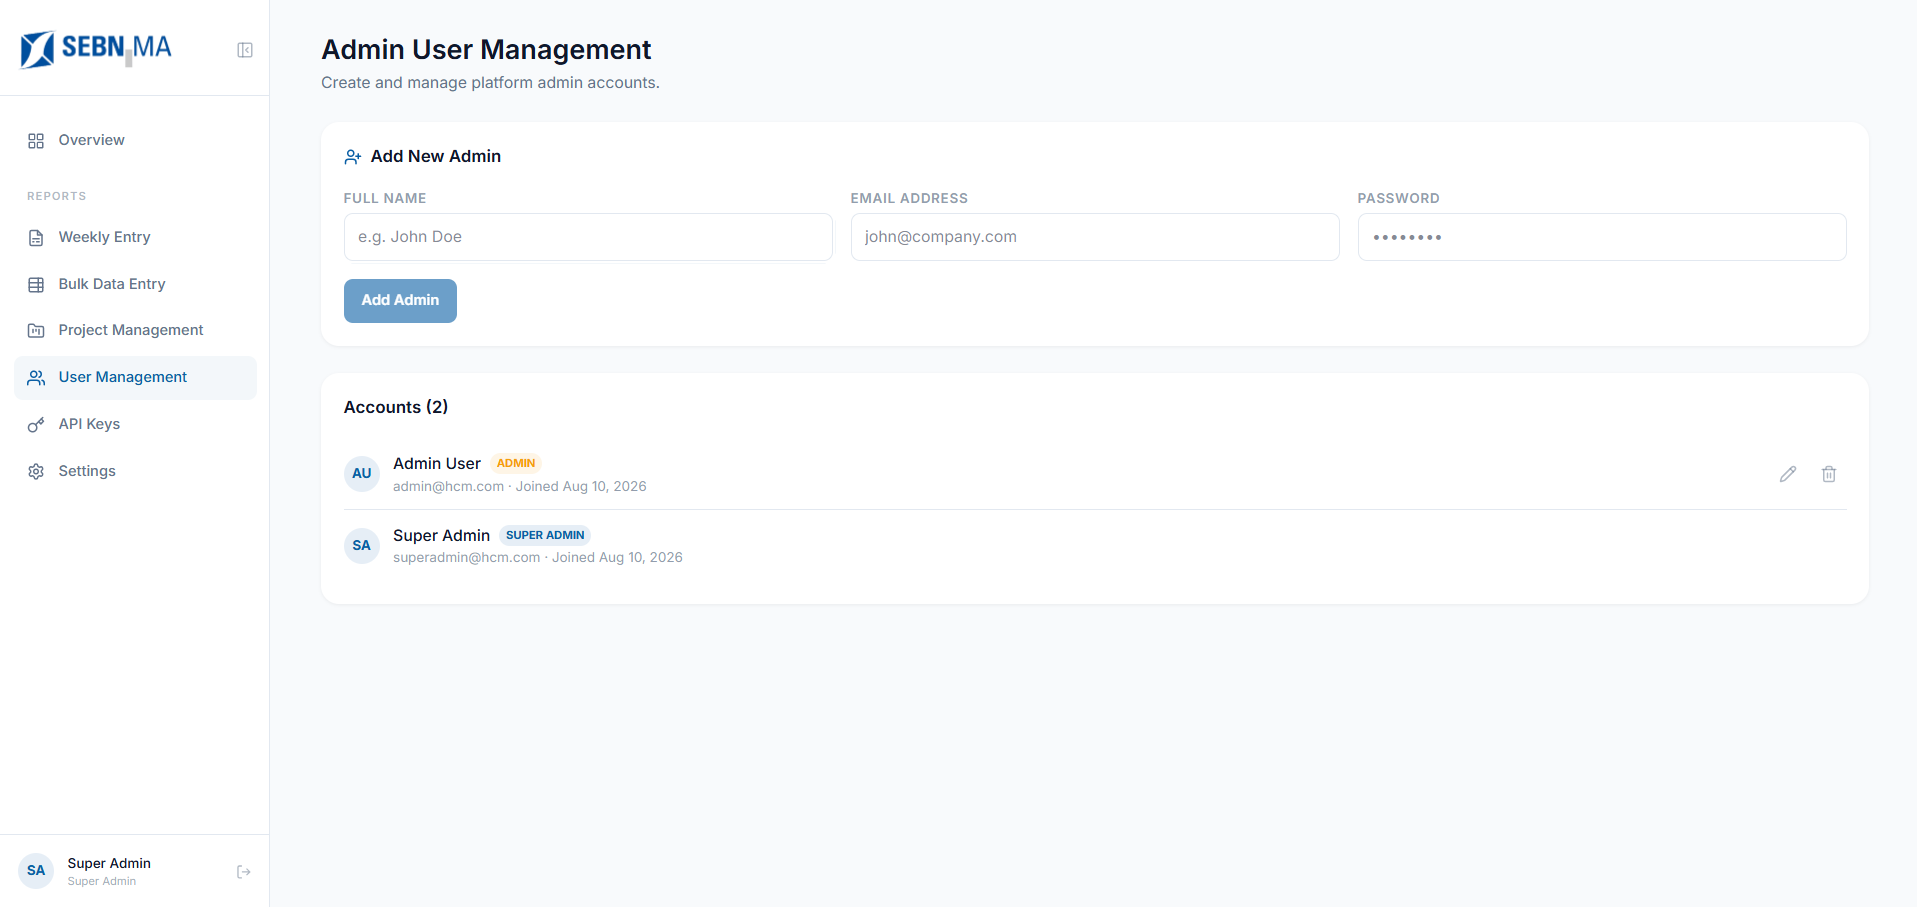
\includegraphics[width=\linewidth]{images/Ch5/users.png}
        \caption{Gestionnaire d'accès et de comptes utilisateurs}
        \label{fig:ui_admin_panel}
    \end{minipage}
\end{figure}

Les panneaux d'administration permettent la création de nouveaux projets, l'attribution des rôles utilisateurs et la génération sécurisée des clés d'API nécessaires à la macro d'automatisation (Phase 2).

% ---------------------------------------------------------
\section{Tests et Assurance Qualité}
Afin de valider la fiabilité de la solution, une stratégie de test rigoureuse a été implémentée. Le Backend est couvert par des tests automatisés via \textbf{Pytest}, s'exécutant sur une base de données SQLite en mémoire. Côté Frontend, \textbf{Vitest} vérifie la robustesse de la logique métier critique (comme le parsing du tableau Excel et le calcul des statistiques des KPIs) avant chaque déploiement.

% ---------------------------------------------------------
\section{Déploiement, Topologie d'Hébergement et Défis Réseau}
\label{sec:deploiement_infra}

\subsection{Topologie de Déploiement Actuelle (Cloud Multi-Plateforme)}
Pour des impératifs d'agilité, de rapidité d'itération et d'optimisation des coûts lors de la phase de validation, l'application a été déployée sur une infrastructure Cloud découplée et multi-fournisseurs :
\begin{itemize}
    \item \textbf{Frontend (Vercel) :} La Single Page Application React est hébergée sur la plateforme \textbf{Vercel}. Elle bénéficie d'un réseau de diffusion de contenu mondial (Edge CDN Anycast) assurant des temps de chargement minimes et un renouvellement automatique des certificats SSL/TLS.
    \item \textbf{Backend (Railway via Docker Hub) :} L'API FastAPI conteneurisée est déployée sur le PaaS \textbf{Railway}. Le service est configuré pour écouter le registre \textbf{Docker Hub}, déclenchant un redéploiement automatique dès qu'une nouvelle image est poussée par le pipeline CI/CD GitHub Actions.
    \item \textbf{Base de Données (Neon Database) :} Les données sont hébergées sur une instance PostgreSQL Serverless gérée par \textbf{Neon}. Cette solution offre une séparation du stockage et du calcul, des sauvegardes automatiques ainsi qu'un chiffrement obligatoire des connexions via SSL (\texttt{sslmode=require}).
\end{itemize}

\subsection{Contraintes du Réseau Industriel SEBN-MA}
Lors des essais d'intégration sur site, une contrainte majeure a été identifiée : la politique de sécurité informatique (IT/OT) de l'usine SEBN-MA impose un filtrage réseau strict par pare-feu (\textit{Firewall}) et proxy d'entreprise.
Les flux sortants vers des domaines publics non référencés (notamment les sous-domaines génériques de développement tels que \texttt{*.vercel.app} ou \texttt{*.railway.app}) sont automatiquement bloqués. 

Par conséquent, les ordinateurs d'atelier connectés au réseau local de l'usine ne peuvent pas communiquer directement avec les services Cloud publics. Cette restriction constitue un obstacle direct pour la \textbf{Phase 2} du projet, où les macros Excel VBA et les scripts d'automatisation situés sur les postes de travail locaux doivent transmettre les enregistrements de production à l'API.

\subsection{Solutions Stratégiques pour la Phase 2 (Mise en Production Industrielle)}
Afin de surmonter ce défi et de concrétiser l'ingestion automatisée en production, deux solutions viables ont été analysées et proposées :

\subsubsection{Solution 1 : Déploiement On-Premise avec Cloudflare Tunnel (Recommandée)}
Cette approche consiste à rapatrier l'hébergement de l'application sur un serveur physique ou une machine virtuelle interne au réseau de l'entreprise via \texttt{docker-compose} (Backend, Frontend Nginx et PostgreSQL). 

Pour rendre l'application accessible à la fois depuis le réseau local de l'usine et depuis l'extérieur (pour les managers nomades), nous préconisons l'usage d'un \textbf{Cloudflare Tunnel} (\textit{cloudflared}) :
\begin{itemize}
    \item \textbf{Sécurité à zéro port ouvert :} Le démon de tunneling établit une connexion chiffrée purement sortante (\textit{outbound}) vers les serveurs edge de Cloudflare. Aucun port entrant (\textit{inbound}) n'a besoin d'être ouvert sur le pare-feu de SEBN-MA, préservant l'étanchéité totale du réseau industriel.
    \item \textbf{Double accessibilité :} Les opérateurs sur site accèdent au tableau de bord via l'adresse IP interne (latence nulle), tandis que les utilisateurs distants y accèdent via un domaine public sécurisé protégé par le WAF (Web Application Firewall) de Cloudflare.
\end{itemize}

\subsubsection{Solution 2 : Domaine Personnalisé d'Entreprise et Whitelisting Réseau}
Si la direction informatique privilégie le maintien de l'hébergement dans le Cloud pour s'affranchir de la gestion d'un serveur local, la démarche suivante sera appliquée :
\begin{itemize}
    \item Remplacement des domaines génériques gratuits par un nom de domaine personnalisé et sécurisé propre à l'organisation (ex: \texttt{kpi-cims.sebn.com}).
    \item Soumission d'une demande de mise sur liste blanche (\textit{Whitelisting}) auprès du département réseau/sécurité de SEBN-MA afin d'autoriser les flux HTTPS vers ce domaine certifié à travers le proxy et le pare-feu de l'entreprise.
\end{itemize}

% ---------------------------------------------------------
\section*{Conclusion}
\addcontentsline{toc}{section}{Conclusion}
Cette phase de réalisation a permis de concrétiser les concepts architecturaux définis précédemment. Le choix d'outils modernes et performants (React, FastAPI, PostgreSQL), couplé à des algorithmes de sécurité avancés, a abouti à une application stable, ergonomique et hautement sécurisée. La solution déployée répond pleinement au cahier des charges de SEBN-MA, ouvrant la voie à une intégration réussie dans le cycle de production.
\cleardoublepage
\phantomsection
\chapter*{Conclusion générale et perspectives}
\addcontentsline{toc}{chapter}{Conclusion générale et perspectives}

\section*{Bilan du Projet}
Le stage de Projet de Fin d'Année effectué au sein de l'entreprise \textbf{SEBN-MA} (site de Tanger Free Zone) avait pour mission principale la modernisation, la fiabilisation et l'automatisation du suivi des indicateurs clés de performance (KPIs) pour les ensembles de production critiques \textbf{HCM-S CIM-3}.

Face aux limites d'un processus historique reposant sur des fichiers Excel isolés, des macros complexes et des manipulations manuelles chronophages, nous avons conçu, développé et déployé une solution logicielle complète, découplée et sécurisée. 

L'ensemble des objectifs fixés pour la \textbf{Phase 1} a été atteint avec succès :
\begin{itemize}
    \item \textbf{Une interface web réactive et interactive :} Développée avec React~19, TypeScript et Tailwind CSS~v4, la plateforme offre aux managers une visualisation dynamique et en temps réel de l'OEE, du Scrap Rate et des performances CIM, enrichie de graphiques chronologiques (Chart.js) et du calcul automatique des écarts statistiques (deltas).
    \item \textbf{Un module de transition fluide (Bulk Data Entry) :} L'outil d'ingestion par copier-coller direct depuis le presse-papiers Excel, doté d'une validation client rigoureuse (détection des anomalies de semaines, sets et valeurs négatives), simplifie drastiquement le quotidien des opérateurs.
    \item \textbf{Un backend asynchrone hautement performant :} Propulsé par FastAPI, SQLAlchemy~2.0 et PostgreSQL (\texttt{asyncpg}), il garantit une ingestion en masse atomique et non-bloquante avec documentation automatique OpenAPI.
    \item \textbf{Une sécurité conforme aux standards de l'industrie :} Mise en place d'une gestion des identités par rôles (Visiteur, Admin, Super Admin), d'un rafraîchissement transparent des jetons JWT (Access/Refresh) via un intercepteur Axios avec file d'attente, et d'un stockage \textit{Zero-Knowledge} (SHA-256) des clés d'API.
    \item \textbf{Une démarche d'assurance qualité industrielle :} Mise en œuvre d'une suite de tests automatisés (151 tests unitaires et d'intégration couvrant le Frontend avec Vitest et le Backend avec Pytest), orchestrée par un pipeline d'intégration continue (CI/CD) sur GitHub Actions avec conteneurisation Docker multi-stage.
\end{itemize}

% ---------------------------------------------------------
\section*{Apports et Valeur Ajoutée pour SEBN-MA}
L'implémentation de cette solution apporte des bénéfices opérationnels concrets pour l'usine :
\begin{enumerate}
    \item \textbf{Gain de temps significatif :} Suppression des tâches manuelles de consolidation et de mise en forme des graphiques, libérant un temps précieux pour l'analyse et la prise de décision.
    \item \textbf{Fiabilité et intégrité de la donnée :} Centralisation dans une base relationnelle persistante avec politique de suppression douce (\textit{Soft Delete}), éliminant les risques de corruption de fichiers ou de pertes d'historique.
    \item \textbf{Réactivité décisionnelle :} Identification instantanée des écarts de cadence et des dérives de rebut sur chaque Set machine grâce aux alertes et aux faits marquants (\textit{Highlights}).
\end{enumerate}

% ---------------------------------------------------------
\section*{Perspectives et Évolutions Futures (Phase 2)}
Bien que le système actuel soit pleinement opérationnel, ce projet pose les fondations de plusieurs perspectives d'évolution majeures :
\begin{itemize}
    \item \textbf{Déploiement On-Premise avec Cloudflare Tunnel :} Afin de s'affranchir des restrictions du pare-feu d'entreprise sans compromettre la sécurité périmétrique, le déploiement local de la stack via \texttt{docker-compose} combiné à un tunnel chiffré unidirectionnel constitue l'étape immédiate pour rendre l'outil accessible sur tout le réseau de l'usine.
    \item \textbf{Automatisation totale du flux d'ingestion (Phase 2) :} Connexion directe des scripts locaux et macros VBA aux endpoints d'ingestion sécurisés via clés d'API, atteignant ainsi une automatisation intégrale « zéro saisie ».
    \item \textbf{Maintenance prédictive et Machine Learning :} Grâce au choix stratégique de l'écosystème Python côté backend, la solution pourra intégrer des modèles d'apprentissage automatique pour anticiper les pannes d'outillage sur les machines HCM-S et prédire l'apparition de micro-arrêts sur les lignes CIM-3.
\end{itemize}

% ---------------------------------------------------------
\section*{Bilan Personnel et Professionnel}
Ce stage au sein de SEBN-MA a constitué une opportunité majeure sur le plan technique et humain. Il m'a permis d'appréhender les réalités et contraintes du secteur automobile (industrie de Rang 1), de maîtriser des technologies modernes de pointe (React~19, FastAPI, Docker, CI/CD), et de piloter un projet de bout en bout, de l'expression des besoins industriels jusqu'au déploiement et à l'assurance qualité.


\end{document}